%
% Example SDSU Mathematics LaTeX Thesis.
% Lines beginning with % are comments and are ignored.
%
% The class file sdsu-thesis.cls must be in the current directory or installed
% with the other classes as per standard LaTeX installation.
%
% To generate run these commands:
%   latex thesis
%   bibtex thesis
%   latex thesis
%   latex thesis
% Then you need to use the dvips command to get postscript output
%
% See the README file for more information

\documentclass{sdsu-thesis}

% For early printouts to save paper use the savepaper option as

%\documentclass[savepaper]{sdsu-thesis}

% This will make things single spaced, use small font and smaller margins.
% Stuff will be formatted differently if you don't use this option but it's
% useful to basically see (read) what you typed so far on paper without
% wasting much paper.  You might want to also comment out the front matter
% and backmatter if printing out in savepaper mode to save paper there.
% Do not use this option on your final printout as it doesn't satisfy the
% thesis manual requirements.

% Also if you want to use double spacing rather then singlespacing (if your
% thesis is very short, say 25 pages or less), then use
% the `doublespace' option as
%\documentclass[doublespace]{sdsu-thesis}

% For pictures, include these
\usepackage{epic}
\usepackage{eepic}
\usepackage{color}
\usepackage{graphicx}
\graphicspath{{figures/}}
% what is natbib anyway?
\usepackage[round]{natbib}

% For chemistry use this.  We've included it because of the chemistry examples.
%\usepackage{dchem}
% For including encapsulated postscript figures use
%\usepackage{epsfig}

% Since this is a math thesis, you quite likely want these:
\usepackage{amsmath}
\usepackage{amsfonts}
\usepackage{amssymb}
\usepackage{amsthm}

% Other useful packages for theses (see LaTeX docs for descriptions of these)
%\usepackage{varioref} % for the \vref commands that also prints out the reference page
%\usepackage{alltt} % for including computer code
\usepackage{url} % for the \url{http://foo.com} command to include url's (or filenames)
\usepackage{longtable} % For multi page tables

% For commutative diagrams.
\usepackage[matrix,arrow]{xy}


% The style of theorems and such that you want to use.  You can change the
% style by modifying the second argument (for example prepending '\sc ' as
% in {\sc Theorem} which will make the headings come out as small caps rather
% then bold)
 \newtheorem{theorem}{Theorem}[chapter]   %Numbered within chapter
 \newtheorem{lemma}{Lemma}[chapter]       
 \newtheorem{definition}{Definition}[chapter]
 \newtheorem{corollary}{Corollary}[chapter]
 \newtheorem{proposition}{Proposition}[chapter]

%  Another option is below.  It uses the same numbering system
%  for the theorems, propositions, lemmas, corollaries and definitions.
%  To see the effect, try compiling twice:  The first time with the
%  set of commands above; the second time comment out those commands 
%  and uncomment the ones below.  
%  The [theorem] entry in the lines below indicates the counter used
%  for theorems will also be used to number propositions, corollaries,etc.
%  Read the LaTeX manual for further explanation.

%
%%  \newtheorem{theorem}{Theorem}[chapter]      %Numbered within chapter
%%  \newtheorem{lemma}[theorem]{Lemma}          
%%  \newtheorem{corollary}[theorem]{Corollary}  
%%  \newtheorem{proposition}[theorem]{Proposition} 
%%  \newtheorem{definition}[theorem]{Definition}

% Author name and the author name in upper case
\author{Charles R. Schmidt}

% Title of the thesis (all in upper case), use \\ for line breaks
% as usual, you can use up to 4 lines and make sure to set the
% counter titlelines to the number of lines you used.
% This is for the title page
\title{EFFECTS OF IRREGULAR TOPOLOGY \\ IN \\ SPHERICAL SELF-ORGANIZING MAPS}
% Number of lines in the title, without setting this the title page
% will not be formatted properly
\setcounter{titlelines}{3}

% Heading style title, the number of lines can be different here then in
% titlelines and in fact the thesis manual requires that this be at most
% 3 lines long so only put at most 2 pagebreaks here.  This is for
% the abstract pages and the signature page.
\titleheading{Effects of Irregular Topology in Spherical Self-Organizing Maps}

% degree
\degree{Master of Science}
% 'Mathematics' for pure maths, and 'Applied Mathematics' for applied
\degreein{Geography}

% If you need to change the word 'Thesis' use \thesisname{Blah} and
% if you need to change the middle line between \degree and \degreein
% on the titlepage to something other then 'in' use \inofand{of} to
% use 'of' for instance

% Dates
\gradyear{2008}
\submitdate{May 2008}

% Your committee chair (don't include titles as per the manual)
\committeechair{Sergio J. Rey}
\committeechairdept{Department of Geography}

% Second committee member
\committeesecond{André Skuin}
\committeeseconddept{Department of Geography}

% Third (usually different department) committee member
\committeethird{Robert P. Malouf}
\committeethirddept{Department of Linguistics and Asian/Middle Eastern Languages}

% Fourth is optional
%\committeefourth{Some Other Person}
%\committeefourthdept{Department of Otherness}

\begin{document}

% Title page (mandatory for SDSU thesis)
\maketitle

% Signature page (mandatory for SDSU thesis)
\makesignature

% If you want a copyright page, give the year and name
% It will be centered vertically and horizontally
% This seems to be mandatory in the revision 11 of the
% SDSU thesis style


\begin{copyrightpage}
Copyright 2008 \\
by \\
Charles R. Schmidt
\end{copyrightpage}

% Dedication (make sure to format this correctly
% including a vspace (say \vspace{3in} or using vfill)
% to make it center on the page if desired, see
% the thesis manual)
% Or just delete this if you don't have a dedication
%\begin{dedication}
%\vspace{3in}
%\centering
%Dedicated to the Utah-Hawaii case.
%Dedicated to quality public education:  May the State of California
%appreciate its value.
%\end{dedication}

% Epigraph (make sure to format this correctly, it
% will just be centered on the page, see the manual)
% Or just delete this if you don't have an epigraph
%\begin{epigraph}
%It's not everyday you see a three man tambourine section,
%it's not everyday,
%because today has been a good day.\\
%\begin{flushright}
%-- Beck
%\end{flushright}
%\end{epigraph}

% Here type the abstract of your thesis.  This is mandatory for
% the SDSU thesis style
%\begin{abstract}
% This just inserts the the abstract.tex file
%% You insert your abstract in the space below.


This document is intended to help students at San Diego State
University to use  \LaTeX\ to produce a Master's Thesis with
high-quality typesetting. Instructions are given for typesetting
complex mathematics and chemical formulas, formatting theorems, using a
variety of table formats, handling figures, and using {\sc Bib}\TeX.  




%\end{abstract}

% Table of contents (this is mandatory in the SDSU thesis style)
\tableofcontents

% If you don't want a list of tables page, delete or comment out
% this line
%\listoftables

% If you don't want a list of figures page, delete or comment out
% this line
%\listoffigures

% Your acknowledgments go here
% Or just delete this if you don't have acknowledgments
% (you should!)
\begin{acknowledgements}
%Sergio J. Rey
%André Skuin
%Robert P. Malouf

%Phil for the writing
%Boris for some ideas
%Maribel for climbing

%And the rest of the Regal team for friendship and support.

%I would like to thank Dr. Gauss for allowing me to work on this
%thesis even though he has been dead for so many years.  I would also
%like to thank Dr. Bolzano for not having any comments on this thesis,
%and I would like to thank Dr. Knuth for being the only living person
%on my thesis committee, and for writing the wonderful \TeX.
\end{acknowledgements}

% This includes body.tex
\chapter{INTRODUCTION}
The Self-Organizing Map (SOM) is an unsupervised competitive learning process
developed by Teuvo Kohonen as a technique to analyze and visualize high
dimensional data sets.  The applications of SOM are far reaching;
\cite{Kohonen2000} provides a thorough review of the SOM literature including
applications of SOM.  SOM has been used in applications ranging from speech
recognition and image classification to breast cancer detection and gene
expression clustering.  \cite{skupin08} outline the growing interest of SOM to
the GISciences, and propose that the relationship between SOM and GIScience
should be bidirectional.  The SOM offers a powerful method for exploring and
visualizing geographic data and GIScience offers a wide array of tools
and methods to enable the exploration of the SOM itself.  The exploration of
spatial relationships has always been of great interest to geographers, and as
\cite{ritter99} states, the goal of SOM is ``to translate \emph{data
similarities} into \emph{spatial relationships}'' \citep[p. 1]{ritter99}.  This thesis leverages
GeoVisualization and GeoCompution in order to explore some of the basic
properties of the SOM.

The SOM is a type of artificial neural network in which neurons are ``organized''
in such a way as to project the high-dimensional relationships of a set of
training data onto a low-dimensional network structure.  The traditional
SOM uses a rectangular or hexagonal network topology \citep{Kohonen2000}.  These topologies 
create a well-known problem in SOM called the boundary or edge effect.  Neurons on
the boundary of the hexagonal and rectangular lattices have fewer neighbors,
which reduces their ability to interact with other neurons during the
self-organizing process.  Using a spherical lattice has been widely suggested as a
solution to the problem \citep{ritter99, boudjemai2003, sangole03,
Nishio:2006fk, wu2006}. The use of the spherical lattice, however, does not
completely overcome the boundary problem, and the choice of which spherical
topology to use for the network can be difficult to make.

A regular network topology is one in which every node on the network has exactly the
same number of adjacent nodes.  Any topology involving an edge is irregular.
Arranging our lattice on the surface of a sphere seems to be an obvious
way to overcome the edge.  However, there exist only five arrangements on the
sphere which are completely regular; these are the five platonic solids \citep{ritter99,
harris2000}.  Any other arrangement of neurons on the surface of the sphere will
result in an irregular topology, as not all neurons will have the same number of
neighbors.  The classic method for minimizing this irregularity is to generate
the spherical lattice by tessellating (subdividing) the sides of the icosahedron
\citep{Nishio:2006fk}.  While this method will always result in a highly
regular spherical topology, the main drawback is that the number of neurons in
the network (the network size), \(N\), grows exponentially as tessellations are
applied. That results in only very coarse control over network size.
 Other methods for arranging neurons on the sphere allow
for unlimited control over network size, but yield topologies with increased
irregularity \citep{harris2000, wu2005, Nishio:2006fk}.  To date the
literature has largely ignored the more irregular methods in favor of the
aforementioned tessellation-based methods.  A topology which yields a more flexible network
size may be desirable.  However, in order to address this issue of network
size, we must first determine the degree to which irregularity effects the
SOM.

\section{Research Objectives}
The objective of this research is to determine the utility of certain irregular
spherical topologies beyond offering greater control over network size.  Toward
that end, we develop and test new diagnostics to measure and visualize
topology-induced errors in SOM.  The following diagnostics are developed and
implemented:

\begin{enumerate}
    	\item Compare the internal heterogeneity of observations captured by a given neuron to that neuron's first-order neighborhood size.
	\item For different topologies, compare the internal heterogeneity of each neuron against a composite measure of topological regularity.
	\item Develop a SOM-based visualization of the internal heterogeneity.
	%\item Develop a reverse quantization error visualization by mapping neurons back onto the input data.
\end{enumerate}

These diagnostics help facilitate the evaluation of both traditional and
spherical SOMs.  To satisfy the objective of this research, we apply these
diagnostics to a series of comparable SOMs.  Each SOM is trained using the
same synthetic data and training parameters, but utilize different network
topologies.  By formally testing for difference of means and variance in the
results of the diagnostics, the following questions are addressed:

%topologies.  By formally testing for statistical differences in the
%results of the diagnostics the following questions will be addressed:
\begin{enumerate}
	\item Does the internal heterogeneity of a neuron decrease as its first-order neighborhood size, or degree, increases?
	\item Is the average internal heterogeneity of a SOM higher when a more irregular topology is used?
	\item Which insights, if any, can be gained from a SOM-based visualization of internal heterogeneity?
\end{enumerate}

\chapter{BACKGROUND}
This chapter is divided into six sections.  Section \ref{bg:som} introduces
the SOM and some of its basic properties.  Next, section \ref{bg:train}
discusses the training process which allows the SOM to represent our input
data.  In section \ref{bg:topo} we explore the importance of topology in the
SOM.  The following two sections, \ref{bg:edge} and \ref{bg:sphere}, expand on
this discussion by introducing some potential problems and possible solutions
found with the traditional topologies used in SOM. Specifically, section
\ref{bg:edge} describes edge effects and section \ref{bg:sphere} describes the
use of spherical topologies which attempt to overcome these edge effects.
Finally, section \ref{bg:size} highlights the importance of the network size
in SOM.



%The first provides a general
%introduction to the SOM algorithm and the problems created by using irregular
%topology. The second reviews the current spherical topologies used with SOMs.
%The third examines the flexibility of the various topologies with regard to
%network size. The fourth takes a look at the limitations of using ``uniformity''
%to evaluate potential topologies.


%Kohonen suggests that a fundamental hierarchy can be found the ``structured occupation and utilization of a uniform memory territory'' \cite[p. 102]{Kohonen2000}.
%Artificial neural networks are a broad class of mathematical or computational models that are conceptually based on biological neural networks.
%The SOM is often classifed as a data reduction technique as it projects a high-dimensional input space onto a low-dimensional lattice, or map, of neurons.
%Kohonen mimics the ``structured occupation and utilization of a uniform memory territory'' that is found in these networks.
%He suggests that the geometric or spatial organization of information in these territories, or spaces, provides for a fundamental hierarchy.
%By creating and implanting a conceptual framework of these spaces and the process which organizes information within them,
% Kohonen is able to represent the similarities of high-dimension information as spatial 
%among input signals as relationships among samples from an input-space as 
%and the process which organizes information within this territory \cite[p. 102]{Kohonen2000}.
%In the SOM an input-space is organized onto a set of neurons through an unsupervised competitive learning process.
%The learning, or training, process organizes information onto this space by presenting input signals to the network.
%Neurons compete for input signals and winning neurons are updated to better model these signals.
%The neurons compete for the input signals and winning neurons updated in order to model them.
%The SOM follows from a conceptual understanding of the process which organizes information within this territory.  
%The neurons act as the uniform memory territory, which is structured by a network topology that defines the connections between these neurons.
%The rectangular and hexagonal topologies shown in Figure \ref{topos} are traditionally used for this purpose.
%As the learning progresses similar input signals are attracted to similar areas of the network.
\section{Self-Organizing Maps}
\label{bg:som}
The SOM is a type of artificial neural network developed by Teuvo Kohonen.  In
the SOM an input-space is organized onto a set of neurons through an
unsupervised competitive learning process \citep{Kohonen2000}. The neurons, arranged on a lattice,
compete for input signals.  The input signals are samples from an input-space.
During training the winning neurons and those around them are updated to
better model these signals. In each step of the training process the winning
neuron is the one most similar to a given input signal.  Traditionally, the
neural lattice, or network, has either a rectangular or hexagonal topology.  As shown in
Figure \ref{topos} these topologies have different properties.  In the
rectangular topology, Figure \ref{topo:rook}, internal neurons are bounded by four
neighbors.  In the hexagonal topology, Figure \ref{topo:hex}, internal neurons are
bounded by six neighbors.  In both topologies, edge neurons have fewer
neighbors.  As the learning progresses, \emph{data similarities} in the
high-dimensional input-space are translated into \emph{spatial relationships}
in the low-dimensional neural network \citep{ritter99}.
%As the learning progresses similar input signals become attracted to similar areas of the network, fulfilling the translation from \emph{data similarities} into \emph{spatial relationships}.

\begin{figure}
\centering
\subfigure[Rectangular Topology]{
  \label{topo:rook}
  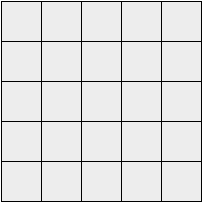
\includegraphics[width=.25\linewidth]{topo_rook.png}
}
\subfigure[Hexagonal Topology]{
  \label{topo:hex}
  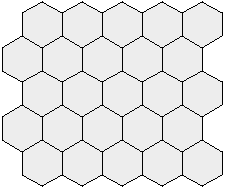
\includegraphics[width=.30\linewidth]{topo_hex.png}
}
\caption{In traditional SOM either a rectangular or hexagonal topology is used.}
\label{topos}
\end{figure}

The SOM has a number of applications, but is primarily used for data reduction
and data visualization.  The SOM is often compared with other data reduction
techniques, such as principal components or multi-dimensional scaling. Like
SOM, these techniques reduce the dimensionality of the input-space
\citep{Kohonen2000,skupin08}. However unlike SOM, these techniques do not
directly perform clustering.  The SOM on the other hand has the ability to do
both simultaneously.  That is the SOM can collapse a high dimensional
input-space into two dimensions, \emph{and} collapse observations from the
input-space into groups or clusters.  The degree to which clustering occurs is
controlled by the size of the SOM.  In smaller SOMs, as the neurons try to
model the input-space, observations are ``collected'' by the neuron which
models it most accurately.  In larger SOMs, perhaps even where there are more
neurons than observations, observations are still collected by their best
model.  However, other neurons map the intermediate areas between
observations, providing a low-dimensional spatial layout of otherwise
high-dimensional data.

\cite{skupin08} demonstrate these properties when they use state level data
from the U.S. Census Bureau to train two SOMs of different sizes.  In the
three-by-three (9) case the neurons act as containers clustering similar
states, while in the twenty-by-twenty (400) case relationships are expressed
with much finer granularity.  In the second case the SOM proves to be a very
useful visualization tool.  The similarities and dissimilarities among the
states are represented as spatial orientations and distances.  Even in this
larger case, where neurons outnumber observations, clustering may still occur.
This happens because the SOM tries to represent the entire input-space.  
The SOM may better represent the input-space by not assigning observations to
every neuron, allowing these neurons to represent dissimilarities, while
clustering of observations occurs at other neurons.

A useful property of the SOM is that the network structure connecting the neurons
allows us to create meaningful visualisations.  Observations used in the
training, as well as new observations from the input space, can be mapped
onto the trained surface in order to show higher dimensional relationships in a
familiar map-like form. The SOM's component planes capture the spatial layout
of each dimension, these are often visualized in a series of maps.  These
maps can provided useful information about the relationships between the
different attributes of your input-space.  In terms of information
visualization, the spatial layout of observations on the network can provide far
more insight than traditional methods, such as ordered lists or scatter
plots.

\section{Training}
\label{bg:train}
% the number of neurons
%and their spatial arrangement are determined before training the SOM.
%An observation from the input space is represented as input vector, \(x\).
%We must also define a distance measure \(d(x,m_i)\) between \(x\) and \(m_i\).
%For this thesis, euclidean distances are used for this purpose.
As with other artificial neural networks, the SOM has to be trained with
samples from the input-space.  These samples, or observations, are represented
as input vectors.  During the training process neurons compete for inputs;
with each training step winning neurons are adjusted to better match the
signals they receive.  Feedback between the neurons allows the entire network to
eventually converge to a final state. After training, each neuron in the SOM
will represent a portion of the input space.  To accomplish this
representation each neuron is associated with a parametric reference vector,
\(m_i\), referred to as a model vector \citep{Kohonen2000}.  The length of each
model vector is equal to the length of the input vectors, such that each
element within a model vector represents a dimension of the input-space.  The
initial values of the elements are most commonly randomized, such that a
mapping of the input-space onto the initial SOM would have no meaning. Other
initializations are possible and may reduce the time required for the map to
converge \citep{Kohonen2000}.

Our implementation follows the ``Original Incremental SOM Algorithm'' as laid
out by \cite{Kohonen2000}.  In each step of the algorithm, a randomly selected
observation (input vector $x$) searches for its best model (reference vector
$m_i$) among the neurons.  The best model is defined as the $m_i$ with the
smallest distance to $x$.  These distances are referred to as quantization
errors (QErrors), and they measure the distance between two vectors in
attribute space \citep{Kohonen2000}.  Our implementation uses Euclidean
distances, however, any reasonable distance measure can be used here.  The
``winning'' neuron is termed the Best Matching Unit (BMU $c$).  The
neighborhood ($N_c$) around the BMU ($c$) is found and all $m_i$ within $N_c$ are
updated.  The size of the neighborhood and the magnitude of the updates are
controlled by the neighborhood function. In our implementation, the width of
the neighborhood decreases as the training progresses, and the magnitude of
the updates decrease, with a Gaussian function, toward the edge of the
neighborhood. A learning-rate factor is used to further reduce the magnitude
of the updates as training progresses.  Combined these create the neighborhood
kernel function $h_{ci}$ which defines a scaler used to adjust the magnitude
of each update in a given training step.  This function always evaluates to
zero for neurons outside the neighborhood.  The update is defined as,
\begin{equation}
  {m_i(t+1)} = m_i(t) +  h_{ci}(t)[x(t) - m_i(t)]
\label{update}
\end{equation}
where, $t$ is the current training step.  The training process is repeated a
predefined number of times, or ideally until the map converges.

\section{Topology}
\label{bg:topo}
%\citeauthor{wu2006} state that ``[f]or SOM, it is desirable to have all
\citeauthor{wu2006} state that ``it is desirable to have all
neurons receive equal geometrical treatment'' \cite[p. 900]{wu2006}.  To
satisfy this constraint, two conditions must be met.  First, each neuron
should occupy the same amount of space on the given surface.  Second, each
neuron should be bordered by the same number of surrounding neurons, and we
should maximize that number.  The first condition is largely irrelevant in the
training of the SOM.  However, visualizations that do not have uniformly sized
and spaced neurons could potentially mislead an untrained viewer, as larger
neurons may appear to be more significant. Of greater importance to
training is the SOM's topology, as it describes how the neurons are connected
within the network.  In training the topology defines, $N_c$, the neighborhood
around the winning neurons, and irregular topologies directly impact the size and
shape of these neighborhoods.  
%According to \cite{wu2006}, the hexagonal structure is more uniform and generally preferred.

We believe the regularity of a given topology, as opposed to spacing and
uniformity, is a better metric
for evaluating different topologies for use in SOM. In graph theory a regular
graph, is simply a graph in which every node has the same number of neighbors
\citep{harris2000}. A measure of regularity tells us how uniform neurons
are in terms of their connections to other neurons in the network. In network
theory, nodes with more connections are thought to be more central to the network and have a
larger influence than nodes with fewer connections \citep{Wasserman:1994}. A simple measure for
capturing this is degree centrality.  The degree (number
of adjacent neurons) is measured for each neuron in the network. The variance
in these measurements tells how regular the network is, a perfectly regular
topology should have a variance equal to zero.  Other methods, such as closeness
centrality compare nodes based on their connectedness to every node in the
network.

\section{The Boundary Effect}
\label{bg:edge}
Traditionally the SOM is laid out on a two-dimensional plane using either a
rectangular or hexagonal topology.  Both of these topologies are irregular,
because neurons on the boundary of the network have fewer neighbors.  Neurons
with fewer neighbors have fewer chances of being
updated \citep{wu2006}.  As observed in Figure \ref{som:states}, neurons in
the center of the map tend to better represent the mean of the input-space.
In this SOM we used the same data as \cite{skupin08} to map the fifty states
and the District of Columbia onto a SOM trained with thirty-two population
census variables. After training, we measured the distance between each
neuron's model vector, $m_i$, and the mean of the input vectors, $\bar{x}$.
Darker neurons have a relatively larger difference from the mean of the input-space,
while lighter neurons are relatively closer. We also measured the difference
of each observation to the mean $\bar{x}$, these distances are represented by
the size of the point symbols.  Larger symbols are farther from the mean. The
five observations furthest from the mean: Alaska, District of Columbia,
Hawaii, Maine, and Utah are highlighted with bold labels.  The five
observations closest to the mean: Alabama, Illinois, Louisiana, Nebraska and
North Carolina have underlined labels.  Arguably the outliers are being pushed
to the edges of the map, where they encounter fewer competing signals.
Edge effects are also common in spatial analysis. For example, in point
patterns the edge of a study unit may hide the true distribution of an
observed pattern.  In SOM, the edge of the neural lattice represents a true
boundary, which effects its ability to represent \emph{data similarities} as
\emph{spatial relationships}.

\begin{figure}[htb]
\centering
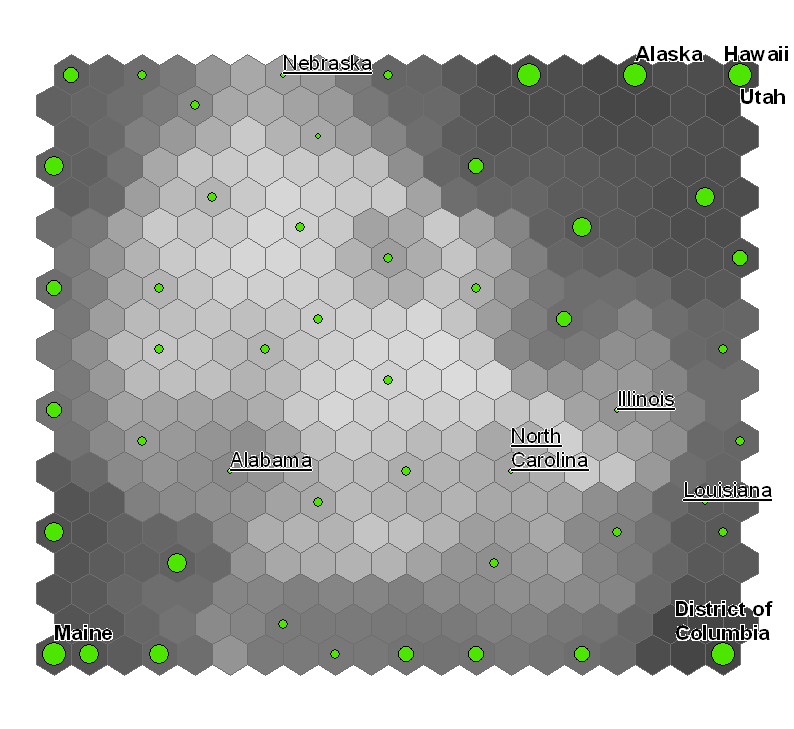
\includegraphics[width=.9\linewidth]{gridedge.png}
\caption{An example of the boundary effect in SOM.}
\label{som:states}
\end{figure}

One way to eliminate the edge effect is to wrap the lattice around a
three-dimensional object such as a sphere or torus, thereby removing the edge
entirely. The toroidal SOM was introduced by \cite{li1993}, however the torus
is not effective for visualization, as maps generated from a torus are not
very intuitive \citep{ito2000,wu2006}.  \cite{ritter99} describes the torus as
being topologically flat and suggests that a curved topology, such as that of
a sphere, may better reflect directional data.  A sphere also results in a
more intuitive map, since we are accustomed to looking at geographic maps
based on a sphere.  

\section{Spherical SOM}
\label{bg:sphere}
\cite{ritter99} first introduced the spherical SOM, and several enhancements have
since been suggested \citep{boudjemai2003,sangole03,Nishio:2006fk,wu2006}.  A
good comparison of these enhancements can be found in \cite{wu2006}.  All of
these methods derive their spherical structure through the tessellation of a
polyhedron as originally proposed by \cite{ritter99}.  \cite{wu2006} point
out the importance of a uniform distribution on the sphere, and that it is
preferable for all neurons to have an equal number of neighbors and to be
equally spaced.  They find generally that the tessellation method best satisfies
these conditions, and specifically that the icosahedron is the best starting
point \citep{wu2005}. Tessellation of the icosahedron results in a network of
neurons, each having exactly six neighbors, save the original twelve
which each have five neighbors.  This is very close to the ideal structure in
which every neuron would have exactly six neighbors.  \cite{wu2006} prefer
this structure, because it has very low variances in both neuron spacing
and neighborhood size. 

Based solely on measures of neuron spacing, \cite{wu2005} dismissed the usefulness of a method
proposed by \cite{Rakhmanov94} for distributing points on a sphere.  Similarly
\cite{Nishio:2006fk} use these variance measures to support their helix
algorithm for distributing points on a sphere.  Table \ref{table1} shows that
these metrics can be misleading and comparison across topologies may not be
consistent.  The traditional rectangular and hexagonal topologies have no
variance in neuron spacing, and the generally preferred hexagonal structure
displays greater variance in neighborhood size than the rectangular structure.
The torus, by comparison, would have variance in neuron spacing, yet no
variance in neighborhood size.  The distance between two neurons is only
considered during the formation of the network topology.  At this stage the
spacing is significant as it plays a part in constructing the network's
topology by determining neuron adjacency.  However, using this measure to
evaluate potential topologies for use in SOM may be misleading.

\begin{table}[htbp]
\caption{Variances in Topologies}
\begin{center}
\begin{tabular}{|c|c|c|c|}
\hline
Topology&Grid Size&Neuron Spacing&Variance in Neighborhood Size\\
\hline
Rectangular&9x18&1&0.2716\\
Hexagonal&9x18&1&1.2138\\
Geodesic&162&0.25319 - 0.31287& 0.0686\\
Rakhmanov&162&0.15779 - 0.30069& 0.2908\\
\hline
\end{tabular}
\end{center}
\label{table1}
\end{table}

As spherical (and other alternative) topologies become
increasingly more common it is necessary to investigate how the choice of
topology effects the SOM.  In this thesis the effect of irregularity within
topologies is studied as an attempt to investigate not only the edge effect,
but also to help facilitate the comparison of topologies.  It is important to
note that spherical topologies may not be appropriate for all applications.
Removing the edge may reduce the SOM's ability to converge.  As outliers are
forced to interact they introduce more competition among the neurons.  We
would also expect outliers to occupy more space in the final map as their
dissimilarity in attribute space should translate to more distant spatial
relationships in the trained SOM.  More research will be needed to help
researchers determine the most appropriate topology for their data and research objectives.

\section{Network Size}
\label{bg:size}
The number of neurons used in the SOM is a decision the researcher must make and
is both a function of the size of their dataset and the purpose for which the
SOM is to be used.  Generally speaking fewer neurons would be used in a
clustering application while larger SOMs are commonly used for visualizing
high-dimensional datasets.  The literature offers little theoretical guidance
on choosing an appropriate network size for a given dataset \citep{cho1996}.
\cite{toolbox} suggests that the network size should be ``as big as
possible,'' but also states that this becomes computationally impractical for
larger problems. As a general rule-of-thumb, \citeauthor{toolbox} suggests using a
network size of \(5\sqrt {n}\), where \(n\) is the number of observations. The
application for which this network size would be most relevant is unclear.  

\begin{figure}[htb]
\centering
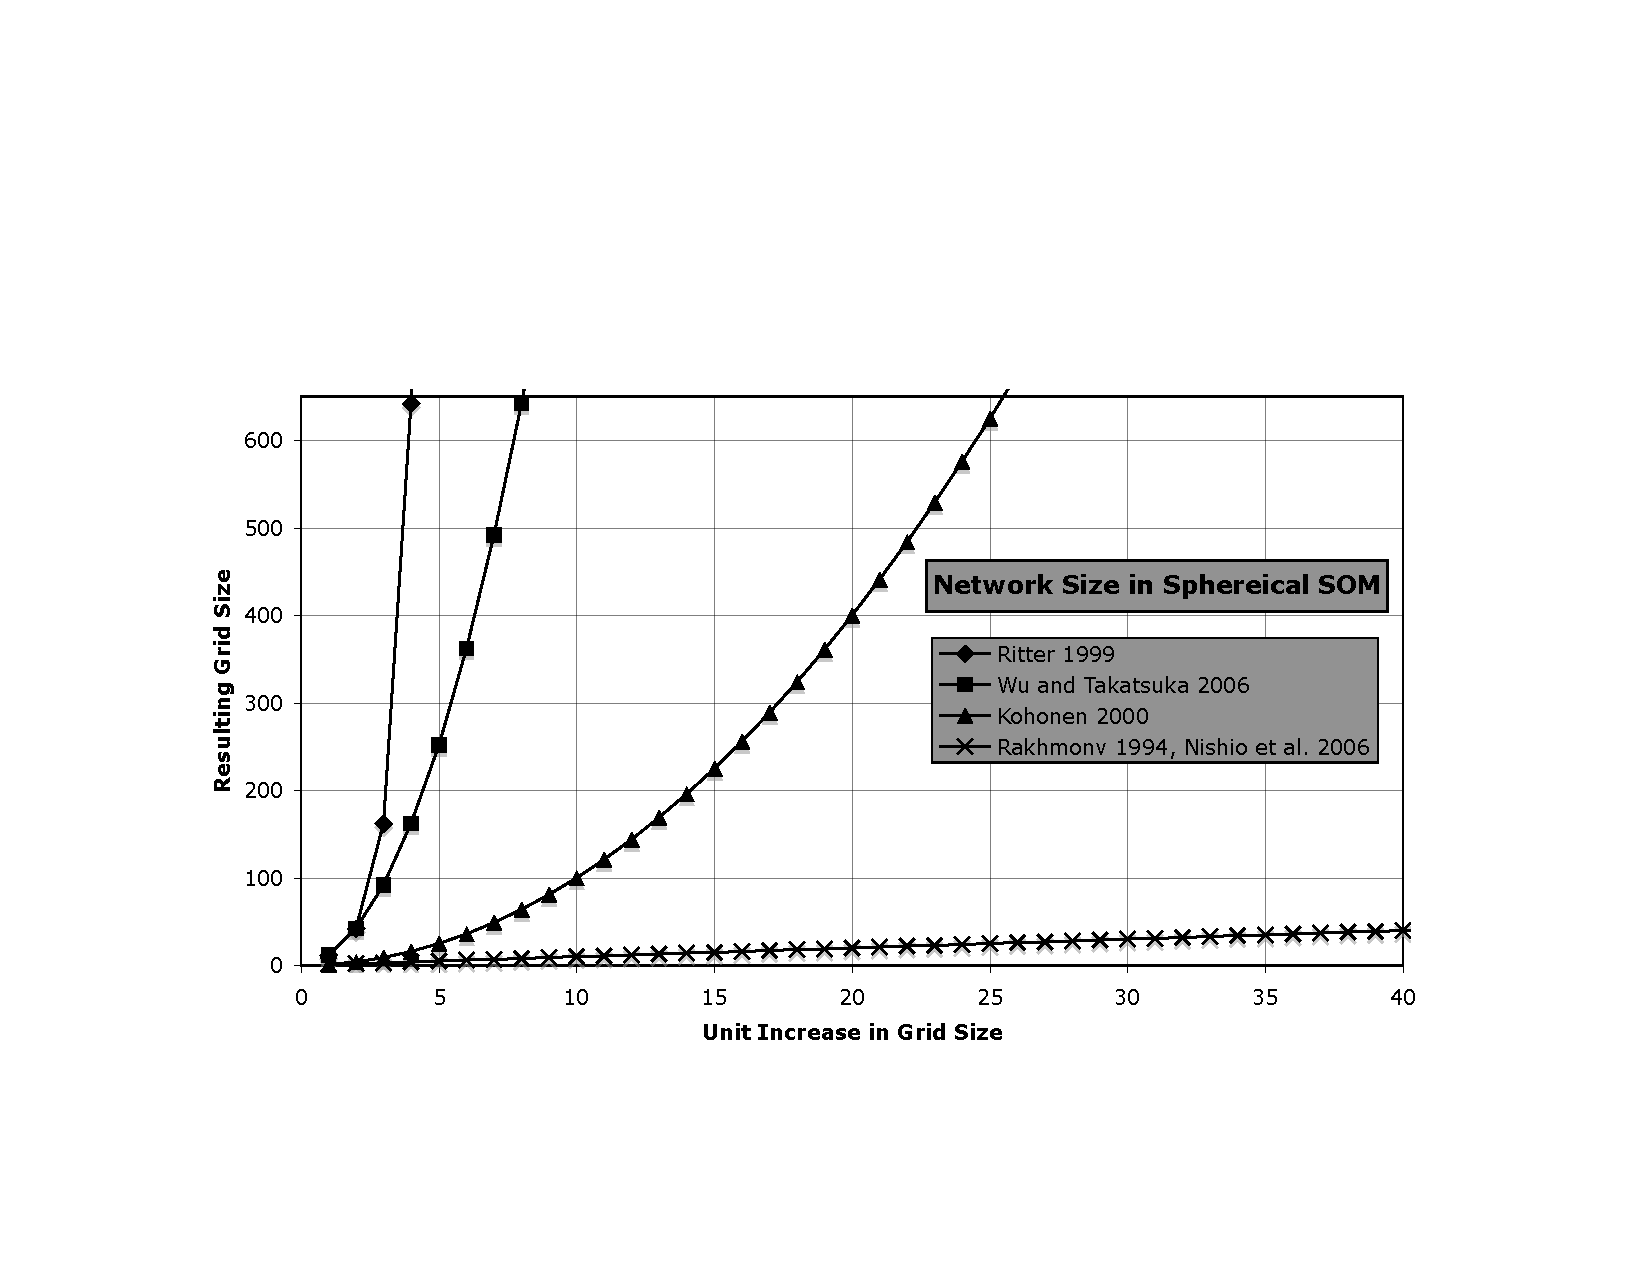
\includegraphics[width=\linewidth]{networkSize.pdf}
\caption{This figure demonstrates the achievable network size using various
spherical topologies, in comparison with the traditional SOM. The Y-axis
represents the achievable network size, while the X-axis represents the
smallest increase in grid size for each topology.}
% frequency of the tessellation. For the traditional Kohonen method the X-axis represents the size of both dimensions of the grid; for comparability the ratio between the dimensions was fixed at one ($X_{dim}=Y_{dim}$).  For the \cite{Rakhmanov94} and \cite{Nishio:2006fk} methods the X-axis represents the exact network size.}
\label{fig:nSize}
\end{figure}

Given this lack of theoretical development, researchers should be cautious
when using methods that limit the control of network size.  Having a high
level of control over network size allows support for such very different SOM
applications as clustering versus low-dimensional spatial layout.
Figure \ref{fig:nSize} shows how the achievable network size varies between
topologies.  In rectangular and hexagonal SOMs it is undesirable to have one dimension
drastically larger than another, as such there are practical limitations to
the size of these networks.  As an aside, the preferred ratio between these
dimensions depends on the data being represented, and should generally not
equal one \citep{kohonen1996, toolbox}.  In Figure \ref{fig:nSize} we used a
ratio of one only for comparison purposes with the other topologies.
\citeauthor{ritter99}'s tessellation method results in a network size that
grows at a rate of \(N=2+10*4^f\), where $f$ is the frequency of tessellation.
\cite{wu2006} offer a slight improvement. Rather than recursively subdividing
the faces, they redivide the original icosahedron with each step, resulting in
\(N=2+10*f^2\).  Methods for arranging an arbitrary number of points on a
sphere provide the highest degree of flexibility when choosing a network
size.  For example, the method proposed by \cite{Rakhmanov94} can
distribute any number of points onto the surface of a sphere.  Strictly
speaking, this is not a topology in itself, as no connections are defined
between the points. In our implementation we create a spherical topology be
applying Delaunay triangulation to these points \citep{Ranka97}.  We refer to
this topology simply as ``spherical''. Using \citeauthor{ritter99}'s method
with a tessellation frequency of three, would result in 642 neurons, the next
smallest size is 162 neurons.  The geodesic topology offers three additional
levels between 162 and 642 neurons (252, 362, 492).  Using the spherical
topology however, we are not limited to these network sizes.

Similarly \cite{Nishio:2006fk} try to address the issue of network size
granularity by departing from the tessellation method and suggesting the use
of a partitioned helix to uniformly distribute any number of neurons on a
sphere.  The method proposed by \cite{Rakhmanov94} was dismissed by
\cite{wu2005} for failing to satisfy the uniformity conditions described
above. \cite{Nishio:2006fk} suggest their method for distributing points
satisfies these uniformity constraints, however they do not describe a network
topology.  It is unclear how they define neighbor relationships and without
clarification we cannot implement their topology.  Methods for distributing
points on the sphere, which allow for fine-grained control over network size,
produce slightly more irregular topologies.  However, no substantive
discussion of these irregularities or their effects on SOM training exists in
the literature. Network size plays an import role in the SOM and given
that limited theoretical guidance is available for choosing network size,
researchers should be cautious when using topologies that limit control over
this parameter.  Particularly for larger SOMs, the desired network size may
not be achievable via tessellation of the icosahedron.


\chapter{METHODOLOGY}
This chapter is composed of four sections.
Section \ref{meth:som} describes PySOM, our own graph based implementation of
SOM. PySOM provides the necessary inputs to our three diagnostics as described
in section \ref{meth:diag}.  These diagnostics were developed to help
understand how irregularities in topology effect the SOM. To use these
diagnostics we must train several SOMs with comparable training data and
parameters.  The specifics of our training data are explained in section
\ref{meth:data}.  Section \ref{meth:train} describes the training parameters used
across all our SOMs.

\section{Graph based implementation of SOM}
\label{meth:som}
The most widely available implementation of SOM is Kohonen's
own SOM\_PAK \citep{kohonen1996}.  SOM\_PAK implements both the traditional
rectangular and hexagonal topologies.  However, implementations of the
geodesic and spherical SOMs were not readily available at the time this thesis
was written.  In order to test these topologies it was necessary to implement
our own version of SOM, PySOM.  Because the goal of this thesis was to study
different topologies for use in SOM, we created PySOM to be topology agnostic.
That is, our implementation is not explicitly aware of the topology.  Rather, we
represent the topology of the SOM as a graph. The graph provides the necessary
information to determine neuron adjacency and construct neighborhoods.  The
nodes in the graph are pointers to the reference vectors ($m_i$).

To allow for rapid development and cross-platform support we choose to write PySOM
in the Python programing language. As noted by \cite{Rey2006} Python is an
object-oriented programing language that is becoming increasingly popular in
scientific computing. PySOM is maintained as an open-source project is hopes
of facilitating collaboration and further research.  In its present form
PySOM has no user interface, however it is written as a Python library which
allows all of its functionality to be accessed programmatically. %spell checked with google

By abstracting the topology, PySOM can train a SOM using any topology for
which a graph structure can be created. We leverage an existing graph library,
NetworkX, to represent our topologies \citep{networkx}.  Our neighborhood
functions are built on top of this library.  Apart from our neighborhood
search functions, our implementation follows the original incremental SOM
algorithm that is described by \cite{Kohonen2000}.  We store our trained SOM
in a similar fashion as SOM\_PAK.  The reference vectors are represented in a
simple text file.  These ``codebook'' files contain a description of the
topology and other training parameters in the first line of the file.  Each
subsequent line lists the values for the parametric reference vectors, $m_i$,
of the SOM's neurons \citep{kohonen1996}. In addition to this codebook file we
also store the graph as a serialized python object.  Creating the graph
structures for the spherical topologies is considerable more complex and
requires more computation than the traditional topologies.

We provide utility functions to create the graph structures for both the
rectangular and hexagonal topologies.  To create the graph structure for the
geodesic topology we use the ``dome'' software package, which outputs the
point coordinates in ``XYZ'' format for each neuron \citep{dome}.  These
coordinates are fed into the STRIPACK software program. STRIPACK computes both
the Voronoi cells and their complement, the Delaunay triangulation, on the
surface of the sphere \citep{Ranka97}.  The Delaunay triangulation provides the graph
structure between the neurons of the geodesic SOM.  A similar process is used
for the spherical topology. In this case we wrote a python implementation of
the method for distributing points on a sphere that was introduced by
\cite{Rakhmanov94}.  Once again the coordinates are fed into STRIPACK.
An additional utility program reads the output from STRIPACK and
creates the NetworkX graph structure.  PySOM has no direct graphical
output, however several utility functions are provided to assist in the
create of visualizations.  These functions create files that are compatible with
popular GIS software packages, namely ESRI's ArcGIS.

\section{Diagnostics}
\label{meth:diag}
In traditional SOMs, outlying observations are pushed to the edge of the map
where they encounter fewer competing signals.  A prime example of this is the
``Utah-Hawaii'' case shown in Figure \ref{som:states}.  Relying only on the
SOM, one would be left to believe that the two states are similar.  Recalling
that the QError measures the distance between two vectors in attribute space,
we see that the QError from Utah to the neuron is $1.509$, the QError from
Hawaii to the neuron in $1.505$, but the QError from Utah to Hawaii is
$3.014$. In this case only Utah and Hawaii were mapped to that neuron.  In a
case where multiple observations land on the same neuron, it is possible to
measure the average pairwise QErrors between those observations.  This gives us a
notion of internal heterogeneity, \(H\), for each neuron.  We define the
internal heterogeneity of neuron \(i\) as,
 \begin{equation}
   {H_i} = \frac{2}{{n_i}^2-{n_i}}\sum_{j=1}^{n_i}\sum_{k=j+1}^{n_i} ||{x_{ij}}-{x_{ik}}||
 \label{eqno1}
 \end{equation}
where, \(n_i\) is the number of observations mapped to \(i\), and \(x_i\) are
the input vectors mapped to \(i\).  For any neuron that captures more then one
observation, this measure tells how dissimilar those observations are.

The edge effects in SOM make it clear that the compression of the input-space is
not uniform through out a trained map.  While outliers being pushed to the edge of
the SOM is not necessarily an undesirable outcome, it is important understand
when and where information is being compressed.  This variable compression of
the input-space is what allows the SOM to represent high-dimensional data, but
it can also mislead the viewer.  Observing the internal heterogeneity of
neurons may shed light on the patterns of compression.  

More specifically we have developed diagnostics that explore how irregularities
in the topology of the SOM effect this internal heterogeneity.  We compare the
internal heterogeneity at the scale of the neuron and the overall map.  Each
diagnostic was designed to answer a specific research question.  The first
diagnostic addresses the research question regarding the internal
heterogeneity and neighborhood size.  The second diagnostic addresses the
question concerning internal heterogeneity and topological irregularity.  The
third helps visualize the patterns between internal heterogeneity; the
usefulness of which is examined in the next chapter.

\subsection{Internal heterogeneity vs. first-order neighborhood size}
\label{q1}
This diagnostic compares the internal heterogeneity of each neuron against
then neuron's first-order neighborhood size.  It would be expected that in
traditional SOMs neurons closer to the edge, those with fewer neighbors, will
have higher internal heterogeneity. Neurons on the edge of the traditional
(rectangular and hexagonal) topologies are considered more irregular, because
they have few neighbors then neurons inside the edge.  This can be extended to
spherical SOMs by considering the degree of any given neuron.  The degree of a
neuron $deg(m_i)$ measures the number of adjacent neurons.  If the
relationship between $H_i$ and $deg(m_i)$ is consistent across topologies,
neurons with lower degrees should display higher internal heterogeneity.

To implement this diagnostic we calculate the internal heterogeneity ($H_i$)
and degree ($deg(m_i)$) of each neuron. The neurons are then separated into a small number of
groups based on the degree.  For most topologies the number of
different degrees will be limited to three or four.  The variance and mean
is calculated for each of these groups.  The expected result is that
variances and means of the groups will decrease as the degree increases.  This
hypothesis is tested using random labeling as described by \cite{siss2004}.
In random labeling, we randomly assign our calculated $H$ values to the
neurons and recompute the mean and variance of the groups.  We do this many times,
9999 in our case, in order to approximate the true distribution. Finally we
calculate pseudo p-values by comparing our observed mean and variance values
with the simulated distributions.  The results are also visualized using
box-and-whisker diagrams. Box-and-whisker diagrams, or box plots, show the
properties of a distribution.  The diagram shows the mean, first and second
standard deviations, and outliers that extend beyond the second deviation.

One problem that we face in this diagnostic is a small sample size when the neurons of a given
SOM are grouped by their degree.  For example, the four corners of the
rectangular topology are the only neurons that have a degree of two.  The rest
of the neurons have three or four neighbors depending on whether or not they
are on the edge. To address the problem of small sample size for topologies
with relatively few neurons of a particular degree, we will increase
the sample size by combining the results of many SOMs.

\subsection{Internal heterogeneity vs. topological regularity}
This diagnostic compares the internal heterogeneity of each neuron against a
measure of regularity for its associated topology.  As mentioned above the
degree of each neuron measures the number of adjacent neighbors.  A completely
regular network topology (i.e. the torus) has no variance between these
measures.  For irregular networks the variance between these degrees gives us
a measure of irregularity. This particular measure is known as degree
centrality.  The degree of a node on a network is a measure of its centrality, or
importance. Nodes with more connections are thought to be more central to the
network and have a larger influence than nodes with fewer connections.

This holds with our understanding of the edge effect.  Neurons on the edge are
less central to the network and have less influence than other nodes.  These
edge nodes are also less influenced by the network, allowing outliers take
root.  During the training process observations that are more average than
others tend to be centralized.  The observations that surround them tend to be
more extreme.  If you refer back to figure \ref{som:states}, you'll notice
that observations with smaller symbols are closer to the mean of the
input-space and that these observations have been centralized in the network.
Using the degree as a measure of centrality does not capture this picture
well, as neurons near the edge can still have a large degree.  A better way to
capture this effect is to look at closeness centrality, which is the
inverse of the average distance of a neuron to every other neuron on the
network.

Closeness centrality provides a more complete measure of connectedness in a
given topology than degree centrality.  In this diagnostic we compare the
internal heterogeneity of the neurons against the average closeness centrality
of their respective topologies.  This results in one group of internal
heterogeneity measurements for each topology tested.  We evaluated this
diagnostic in much the same way as the last.  We compare the variances and
means of each group, testing for differences with random labeling.  It is
expected that the distribution of internal heterogeneity will be narrower for
groups trained on more regular topologies.  It is further hypothesized that
the mean of internal heterogeneity will decrease when the network is more
regular.  In addition to testing these assumptions with random labeling we
visualize the results with box plots.

\subsection{Visualize internal heterogeneity mapping}
Visualizing the internal heterogeneity may yield insight into how irregular topology
effects the SOM.  Creating these visualization for many different topologies
however, offers a number of challenges.  While the rectangular and hexagonal
topologies are rather straight forward to visualize, the spherical and geodesic
topologies are significantly more involved.  In order to leverage the utility
of existing GIS software we represent our topologies in a form that
these software packages understand.  Toward that end we create polygon layers
in which each polygon represents a neuron.  Shared borders represent
connections between neurons.  Creating the polygons for these topologies
required that we first compute the Voronoi diagram on the surface of the
sphere.  This is done using STRIPACK, a software program created by
\cite{Ranka97}.  Despite the prevalence of spherical coordinates
in GIS, modern GIS software packages have their roots in CAD software. As such
they all assume Cartesian distances and thus can not handle polygons that
cross the $180^{th}$ meridian.  To accommodate this we split each polygon at
the $180^{th}$ meridian and redraw it as two parts.

Once the GIS layers have been created and the internal heterogeneity of each
neuron has been calculated, a number visualizations become possible. We
visualize the internal heterogeneity by shading the corresponding polygons.
These visualizations allow for the exploration of patterns in internal
heterogeneity with relation to the underlaying topology.  Further we can
visualize the component planes, which show how the higher dimensions are
represented in the various SOMs.  We also map our synthetic data back onto the SOM in
order to calculate cluster membership of the neurons.  Visualizing cluster
membership clearly shows how the various topologies perform clustering.


\section{Data}
\label{meth:data}
%Comment from Skupin...
%This section is obviously leaving most of the specifics of the synthetic data
%generation out, which is problematic. I'm willing to go along with this for
%the proposal though, unless it gets raised by the third committee member
Our internal heterogeneity measure is sensitive to both the properties of the SOM
and the properties of the training data. Therefore, a dataset with uniform
properties is needed. We follow the method for generating uniform synthetic
data used by \cite{wu2006}.  Their method creates seven clusters in three
dimensions.  Each cluster is normally distributed and has a standard deviation
of one.  The clusters are centered at the origin and ten units out in each
directions on the x, y and z axes. The uniform clusters generated by this method allow us to
systematically compare the diagnostics under several different topologies.  To
ensure that we can calculate an internal heterogeneity for as many neurons as
possible, we create approximately $25,000$ observations in each dataset.  As
described in the next section, our SOMs have either 642 or 644 neurons
(depending on the topology).  Having a large number of observation relative to
the number of neurons will force the SOM to preform clustering, increasing the
number of neurons for which the internal heterogeneity can be computed.

As mentioned in section \ref{q1} we will need to combine the results of
multiple SOMs in order to ensure a large enough sample size.  To accomplish
this we will create ten synthetic datasets as described above.  Each of these
datasets can be thought of as samples from the same input space.  That is, the
data generating process remains the same for each synthetic dataset created.
After training ten SOMs for each topology we take the average internal
heterogeneity of each to ensure that the results are comparable.


%We will create a number of different data sets and use them to train various SOMs.  

%the data is generated in such a way to increase the probability that each neuron will be occupied by more than one observation.

%Initially the synthetic data for this thesis came from a Gaussian cluster
%generator which creates clusters by randomly sampling from multivariate
%normal distributions \citep{handl}.  \citeauthor{handl}' method to keep
%clusters from overlapping is to create one cluster at a time, with each new
%cluster checked to see if it overlaps with an existing cluster. If it does,
%it is rejected.  The generator continues until the desired number of
%non-overlapping clusters has been reached.  This method tends to create
%clusters of very different shapes and sizes (or extents).

%The limit to using this method for creating data became evident when we
%realized that the internal variance measure was being affected by the
%structure of the clusters.  The internal variance essentially looks at the
%portion of a cluster that is mapped to a particular neuron and measures the
%density.  Because we specify that each cluster contain an equal number of
%observations, they tend to get equal representation (in terms of number of
%neurons) on the trained SOM.  The result of all this is that the smaller,
%more dense clusters display very low internal variance relative to the
%larger, less dense clusters.  While this may have interesting consequences in
%other applications, because of these effects on the internal variance our
%ability to determine how changes in the topology are affecting the meassure.
%because it interferes with the measurement of internal variance, we had to
%adopt another method of synthetic data generation. 



\section{SOM Training}
\label{meth:train}
Before we can go on to address the research questions we need to train a
series of SOMs.  We train SOMs using four different topologies:
\emph{rectangular, hexagonal, geodesic sphere} and \emph{spherical}.  The spherical
topology is based on a method, developed by \cite{Rakhmanov94}, for
distributing an arbitrary number of points on to the surface of a sphere.
Delaunay triangulation is then applied to these points, producing a
topological structure.  To yield meaningful results these SOMs must be trained
with comparable parameters.  The literature provides many rules of thumb for
training a SOM: each SOM is trained in two stages, the first of which uses a larger
initial learning rate and neighborhood search radius with a small number of
training steps; the second stage uses a lower initial learning rate and
neighborhood search radius, but extends the length of training.
\\
First Stage Parameters:
\begin{itemize}
  \item Initial neighborhood search radius of 50\%, which decreases during training. 
  \item Initial learning rates of 0.04 which decreases during training.
  \item 100,000 training steps.
\end{itemize}
Second Stage Parameters:
\begin{itemize}
  \item Initial neighborhood search radius of 33\%, which decreases during training. 
  \item Initial learning rates of 0.03 which decreases during training.
  \item 1,000,000 training steps.
\end{itemize}

As shown in Figure \ref{fig:nSize}, topologies differ in terms of achievable
network size.  For comparability, the network size of each SOM needs to be as
close as possible.  The achievable network size for the geodesic SOM is the
most limiting of the topologies we test. We chose the eighth frequency
geodesic sphere, which has 642 nodes, which is relatively close to the
644-node hexagonal and rectangular topologies achieved when the dimensions are
set to \(28x23\). Finally, the spherical topology was set to 642 nodes.




\chapter{RESULTS AND DISCUSSION}
This chapter describes the implementation and results of the empirical analysis
outlined above.  Each section of this chapter details one of the three main
tasks of the empirical analysis.  The first task is to create synthetic data,
the second to train the SOMs and finally to apply the diagnostics.

\section{Data}
%The data will be generated with the common technique of rejection sampling,
%where n high dimensional seeds are chosen at random, samples will be taken
%at random from a uniform distribution, if the sample falls with in radius r of
%any seed it is accepted, if it does not, single random number is drawn, if that
%number is \(<\) 0.05\% the sample is accepted as noise, else the sample is rejected.
The training data will be generated using a Gaussian cluster generator as
described by \cite{handl}.  To generate the data we have to decide how many
clusters to create and how many dimensions to use.  In order to set these
parameters appropriately we will first explore how the internal variance
responds to adjustments in their value.

To accomplish this twenty test data sets are generated and used to train both
the rook and spherical SOMs. As shown in tables \ref{ivtable1} and
\ref{ivtable2} and \ref{ivtablehex} and \ref{ivtablegeodesic} both topologies seem to respond similarly. The internal
variance of the SOM increases as we add dimensions and decreases as we add
clusters. Based on these tables, it was decided that five dimensions and ten
clusters was a reasonable choice. Five dimensions is easier to work with than
larger numbers and should yield more information than two dimensions. 


\begin{table}
\centering
\caption{Mean Internal Variane for the entire som GRAPH}
\label{ivtable1}
\begin{tabular}{|c||c|c|c|c|}
\hline
&\multicolumn{4}{c|}{\textbf{Dimmensions}}\\
\textbf{Clusters} & \multicolumn{1}{c}{\textbf{2}} &
\multicolumn{1}{c}{\textbf{5}} & \multicolumn{1}{c}{\textbf{10}} &
\multicolumn{1}{c|}{\textbf{20}}\\
\hline
\hline
\textbf{0} & 0.0207& 0.2661& 0.7131& 1.3997 \\
\hline
\textbf{2} & 0.0106& 0.1106& 0.2550& 0.4872 \\
\hline
\textbf{5} & 0.0117& 0.0968& 0.2194& 0.4557 \\
\hline
\textbf{10} & 0.0118& 0.0839& 0.2051& 0.4174 \\
\hline
\textbf{20} & 0.0123& 0.0844& 0.1989& 0.4017 \\
\hline
\end{tabular} \end{table}


\begin{table}
\centering
\caption{Mean Internal Variane for the entire som ROOK}
\label{ivtable2}
\begin{tabular}{|c||c|c|c|c|}
\hline
&\multicolumn{4}{c|}{\textbf{Dimmensions}}\\
\textbf{Clusters} & \multicolumn{1}{c}{\textbf{2}} &
\multicolumn{1}{c}{\textbf{5}} & \multicolumn{1}{c}{\textbf{10}} &
\multicolumn{1}{c|}{\textbf{20}}\\
\hline
\hline
\textbf{0} & 0.0206& 0.2796& 0.7300& 1.4173 \\
\hline
\textbf{2} & 0.0114& 0.1140& 0.2598& 0.4930 \\
\hline
\textbf{5} & 0.0116& 0.0989& 0.2213& 0.4623 \\
\hline
\textbf{10} & 0.0117& 0.0873& 0.2071& 0.4207 \\
\hline
\textbf{20} & 0.0120& 0.0851& 0.2020& 0.4059 \\
\hline
\end{tabular} \end{table}

\begin{table}
\caption{Mean Internal Variane for the entire som HEX}
\label{ivtablehex}
\begin{tabular}{|c||c|c|c|c|}
\hline
&\multicolumn{4}{c|}{\textbf{Dimmensions}}\\
\textbf{Clusters} & \multicolumn{1}{c}{\textbf{2}} &
\multicolumn{1}{c}{\textbf{5}} & \multicolumn{1}{c}{\textbf{10}} &
\multicolumn{1}{c|}{\textbf{20}}\\
\hline
\hline
\textbf{0} & 0.0205& 0.2784& 0.7336& 1.4192 \\
\hline
\textbf{2} & 0.0109& 0.1134& 0.2585& 0.4930 \\
\hline
\textbf{5} & 0.0111& 0.0997& 0.2229& 0.4598 \\
\hline
\textbf{10} & 0.0114& 0.0917& 0.2085& 0.4236 \\
\hline
\textbf{20} & 0.0117& 0.0860& 0.2008& 0.4041 \\
\hline
\end{tabular} \end{table}



\begin{table}
\caption{Mean Internal Variane for the entire som GEODESIC}
\label{ivtablegeodesic}
\begin{tabular}{|c||c|c|c|c|}
\hline
&\multicolumn{4}{c|}{\textbf{Dimmensions}}\\
\textbf{Clusters} & \multicolumn{1}{c}{\textbf{2}} &
\multicolumn{1}{c}{\textbf{5}} & \multicolumn{1}{c}{\textbf{10}} &
\multicolumn{1}{c|}{\textbf{20}}\\
\hline
\hline
\textbf{0} & 0.0207& 0.2657& 0.7140& 1.3981 \\
\hline
\textbf{2} & 0.0111& 0.1110& 0.2553& 0.4870 \\
\hline
\textbf{5} & 0.0112& 0.0966& 0.2204& 0.4546 \\
\hline
\textbf{10} & 0.0117& 0.0789& 0.2058& 0.4183 \\
\hline
\textbf{20} & 0.0120& 0.0857& 0.1995& 0.3994 \\
\hline
\end{tabular} \end{table}






\section{Internal variance vs. first-order neighborhood size}
As outlined in section \ref{q1} we can look at how the internal variance
changes with with respect the degree of a neuron.  

In order to compare the IV accross groups it it necessary to train multiple
soms 
To setup this experiment we
first generate ten synthetic data sets using the method desribed above.  These
data sets will be used to train ten SOMs for each topology.  The reason we
train multiple SOMs for each to is to ensure that we have large enough groups to 
As mentioned in section \ref{q1} the neurons.
With these parameters chosen ten data sets are generated and used to train
SOMs for each topology.  After running ten simulations for the spherical,
hexagonal and rook topologies we find that the mean internal variance seems to
remain fairly stable, this suggests that we can combine the results of each
simulation to compare across topologies. As shown in table \ref{ivtable3}.

\begin{table}
\centering
\caption{Mean IV for each simulation, by topology}
\label{ivtable3}
\begin{tabular}{|c||c|c|c|c|}
\hline
\textbf{Simulation Number} & Geodesic & Graph & Hex & Rook \\
\hline
\hline
\textbf{1} & 0.0966 & 0.0968 & 0.0997 & 0.0989 \\
\hline
\textbf{2} & 0.0875 & 0.0874 & 0.0887 & 0.0886 \\
\hline
\textbf{3} & 0.0807 & 0.0809 & 0.0813 & 0.0814 \\
\hline
\textbf{4} & 0.0816 & 0.0812 & 0.0834 & 0.0823 \\
\hline
\textbf{5} & 0.0912 & 0.0907 & 0.0927 & 0.0929 \\
\hline
\textbf{6} & 0.0943 & 0.0938 & 0.0966 & 0.0944 \\
\hline
\textbf{7} & 0.0905 & 0.0908 & 0.0916 & 0.0929 \\
\hline
\textbf{8} & 0.0789 & 0.0792 & 0.0798 & 0.0797 \\
\hline
\textbf{9} & 0.0984 & 0.0974 & 0.0994 & 0.1001 \\
\hline
\textbf{10} & 0.0900 & 0.0897 & 0.0917 & 0.0910 \\
\hline
\end{tabular} \end{table}



%Currently implemented are the rectangular and spherical topologies, the hexagon
%and geodesic are to be implemented only as graphs.  I.E. the topologies will be
%generated externally and turned into a networkX graph, for use in the graph
%based SOM. The spherical topology also relies on external programs to generate
%the graph structure (spherical voronoi).
\subsection{Restate the Questions}
\textbf{Objective}, Compare the internal variance of observations captured by a given
neuron to that neuron's first-order neighborhood size.

\textbf{Question}, Does the internal variance of a neuron decrease as its first-order
neighborhood size, or degree, increases?



this table shows the means and variances for the degree groups,
\ref{meanvar1}. \footnote{The Combined sizes may not add up to expeded amount.
This is because we can only calculate an IV for neurons which are the BMU of
two or more observations.}

\begin{table}
\caption{Mean IV grouped by a neurons degree for each topology}
\label{meanvar1}
\begin{tabular}{|c||c|c|c||c|c|c||c|c|c||c|c|c|}
\hline
\textbf{Degree Size} & \multicolumn{3}{c||}{\textbf{Geodesic}} &
\multicolumn{3}{c||}{\textbf{Graph}} & \multicolumn{3}{c||}{\textbf{Hex}} &
\multicolumn{3}{c||}{\textbf{Rook}} \\
\hline
& N & MeanIV & VarIV & N & MeanIV & VarIV & N & MeanIV & VarIV & N & MeanIV &
VarIV \\
\hline
2&&&&&&& 20& 0.1109& 0.0010& 40& 0.1123& 0.0007\\ 
3&&&&&&& 223& 0.1054& 0.0010& 918& 0.0997& 0.0009\\ 
4&&&&&&& 507& 0.0980& 0.0009& 5138& 0.0875& 0.0009\\ 
5& 115& 0.0898& 0.0009& 557& 0.0886& 0.0009& 208& 0.0921& 0.0008&&&\\ 
6& 5929& 0.0884& 0.0009& 5034& 0.0883& 0.0009& 5184& 0.0881& 0.0009&&&\\ 
7&&&& 437& 0.0873& 0.0009&&&&&&\\ 
\hline 
Combined& 6044& 0.0884& 0.0009& 6028& 0.0882& 0.0009& 6142& 0.0897& 0.0010&
6096& 0.0895& 0.0009\\ 
\hline
\end{tabular} \end{table}




here are the box plots for the IV. \ref{fRookIV} \ref{fGraphIV} \ref{fHexIV}
\ref{fGeodesicIV}


\begin{figure}
\centering
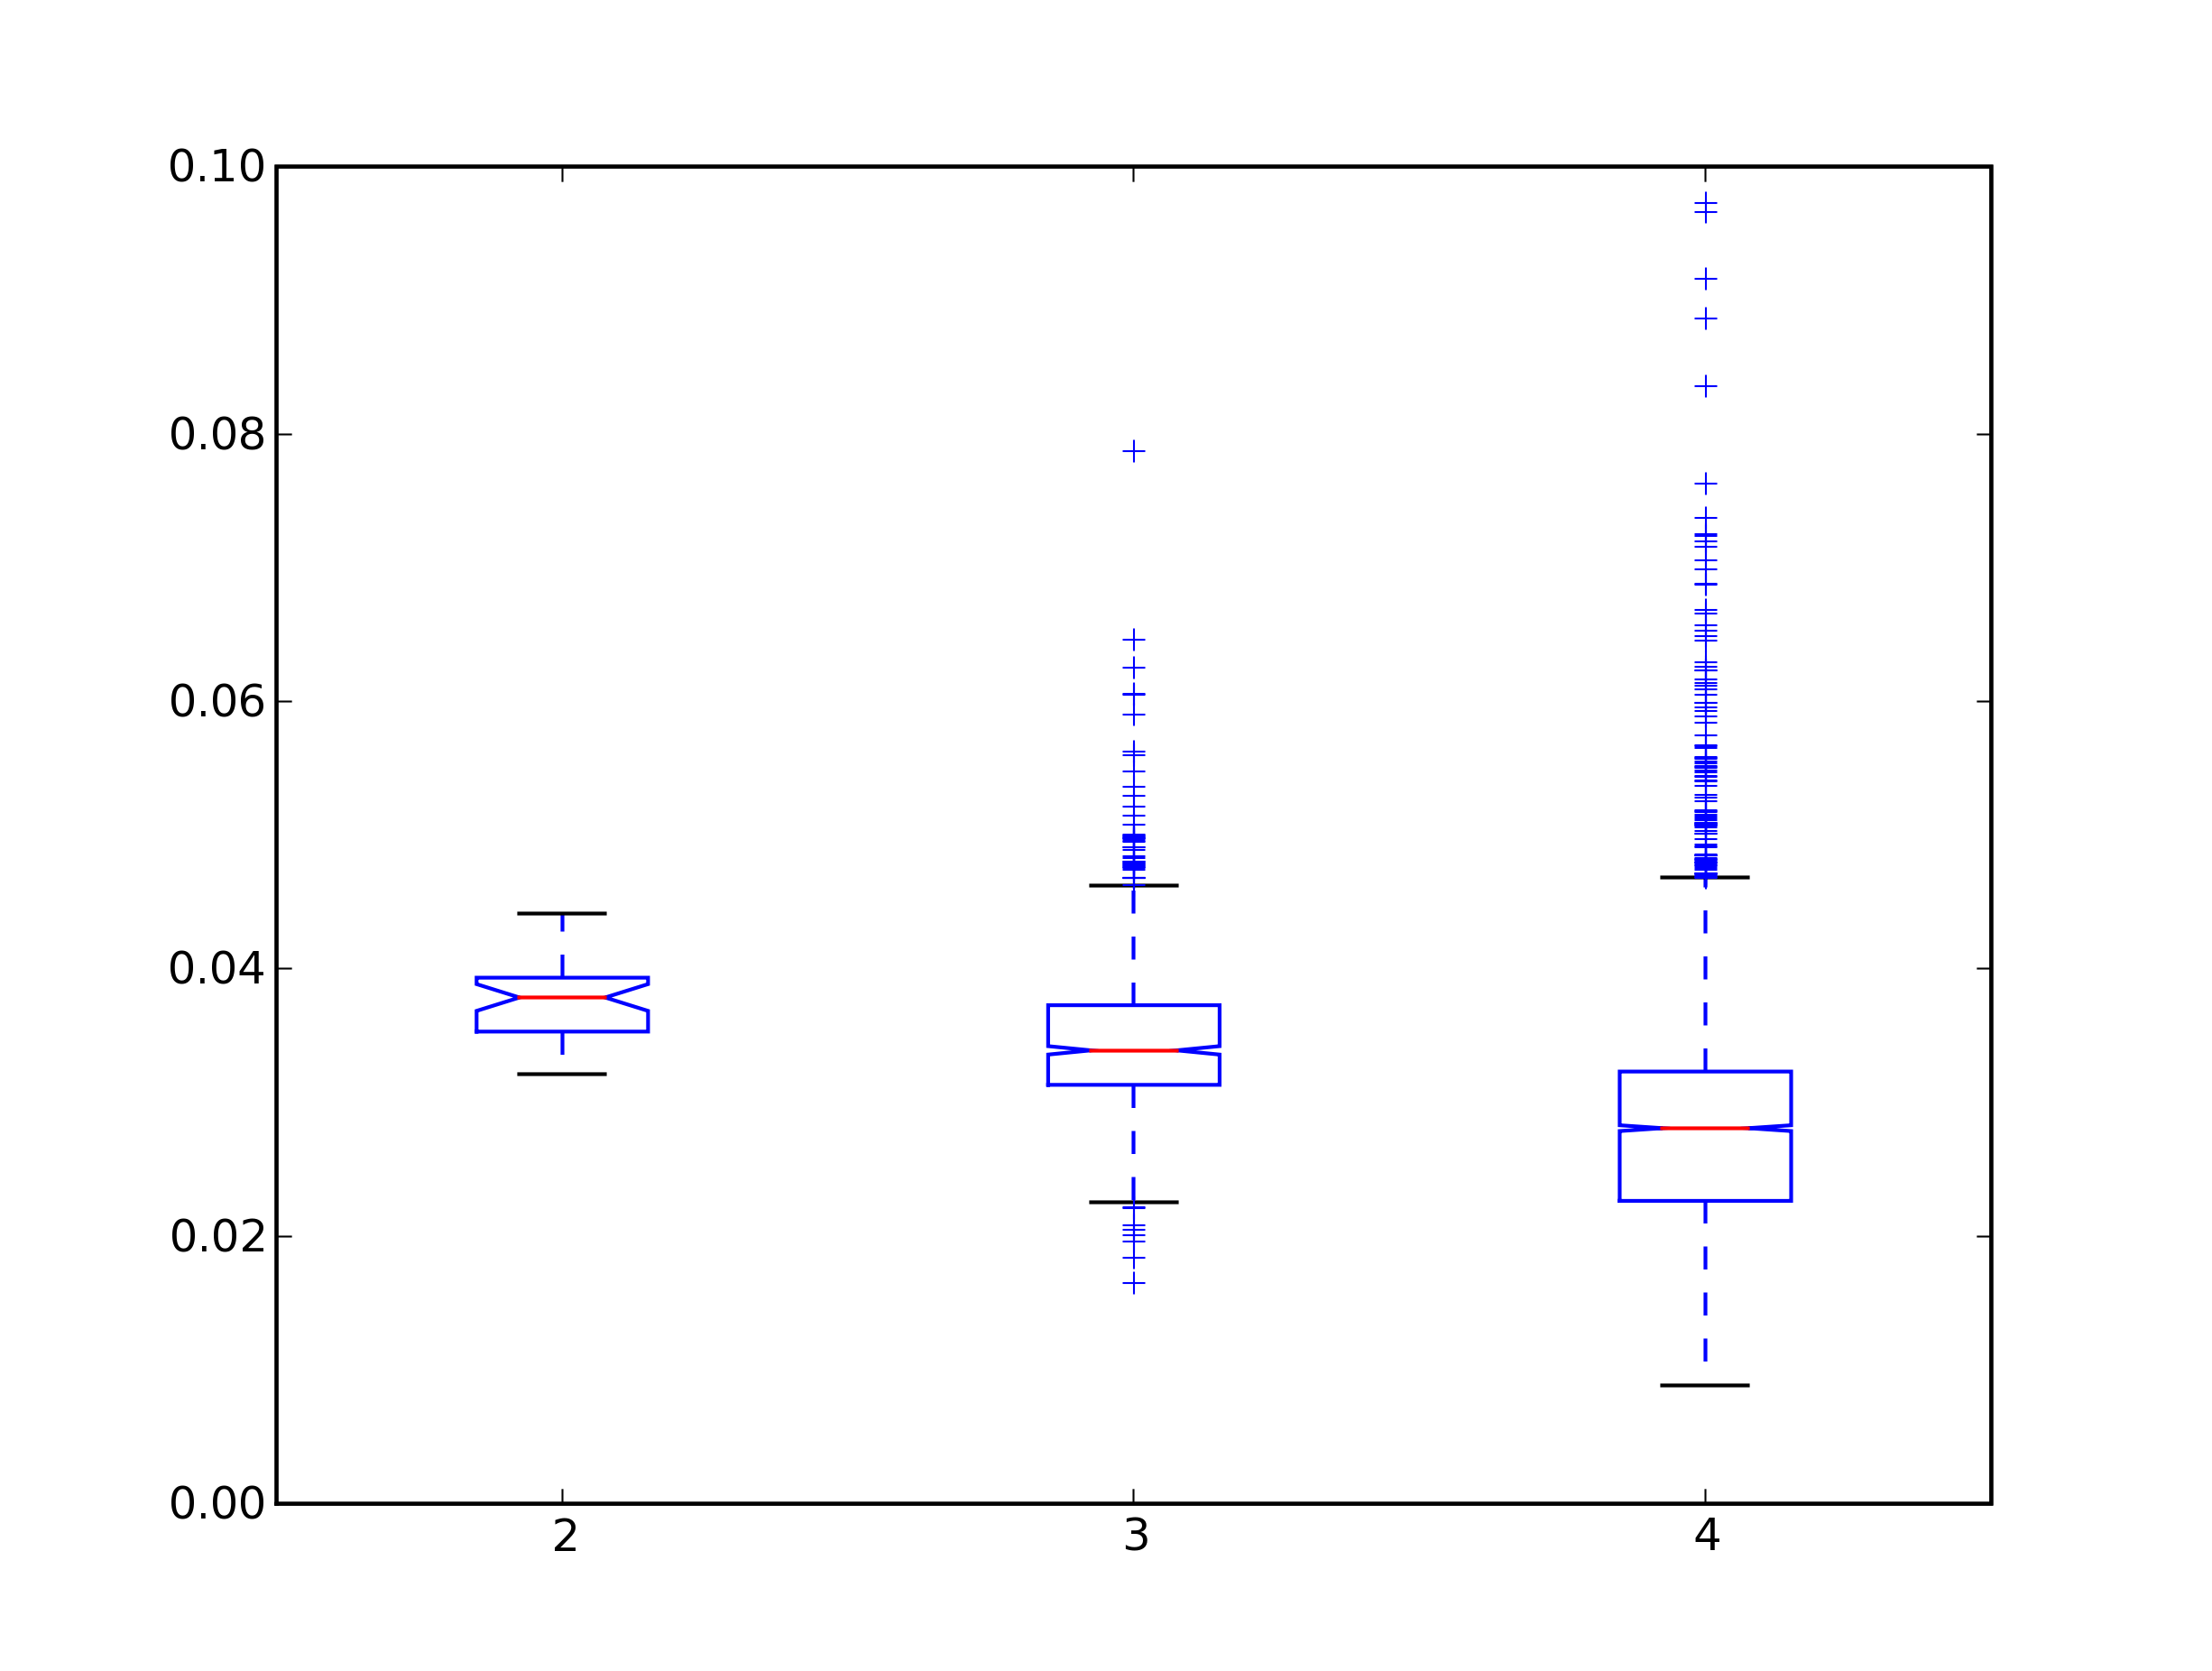
\includegraphics[width=\linewidth]{rook_iv_box.png}
\caption{This shows 4 box plots, each representing one group of neurons in a set
of SOMs trained with the same paremeters.}
\label{fRookIV}
\end{figure}

\begin{figure}
\centering
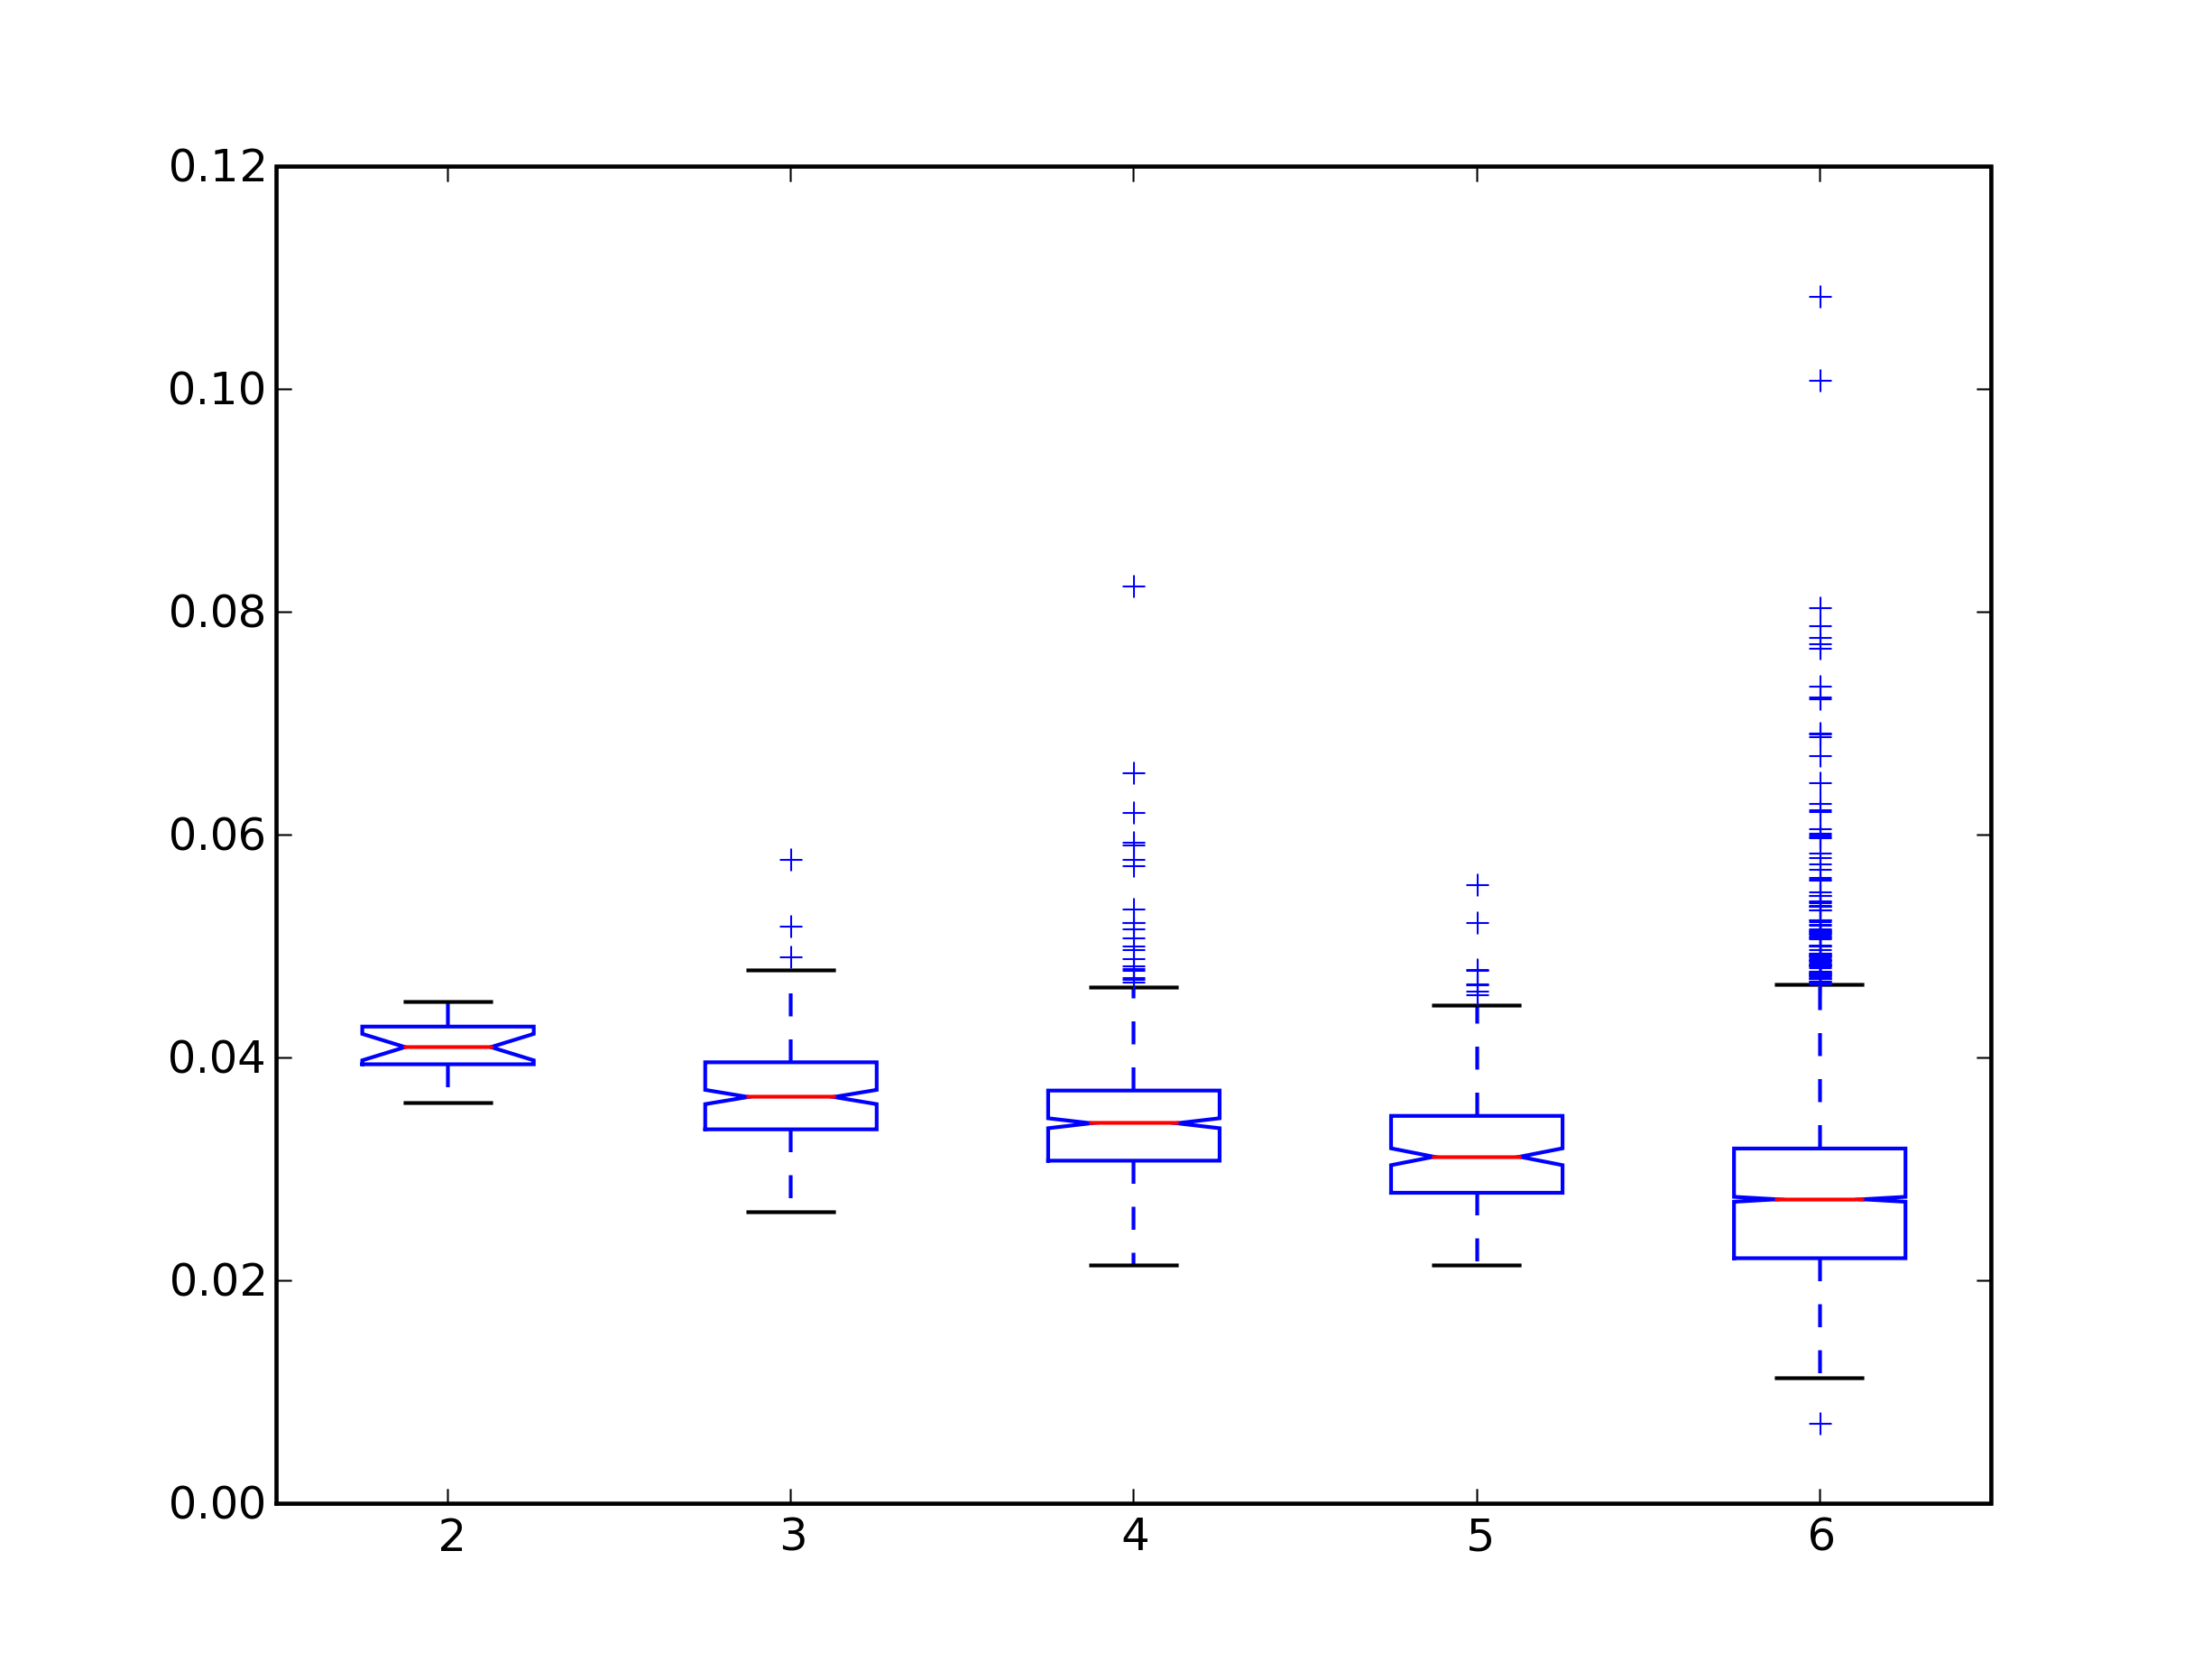
\includegraphics[width=\linewidth]{hex_iv_box.png}
\caption{This shows 4 box plots, each representing one group of neurons in a set
of SOMs trained with the same paremeters.}
\label{fHexIV}
\end{figure}

\begin{figure}
\centering
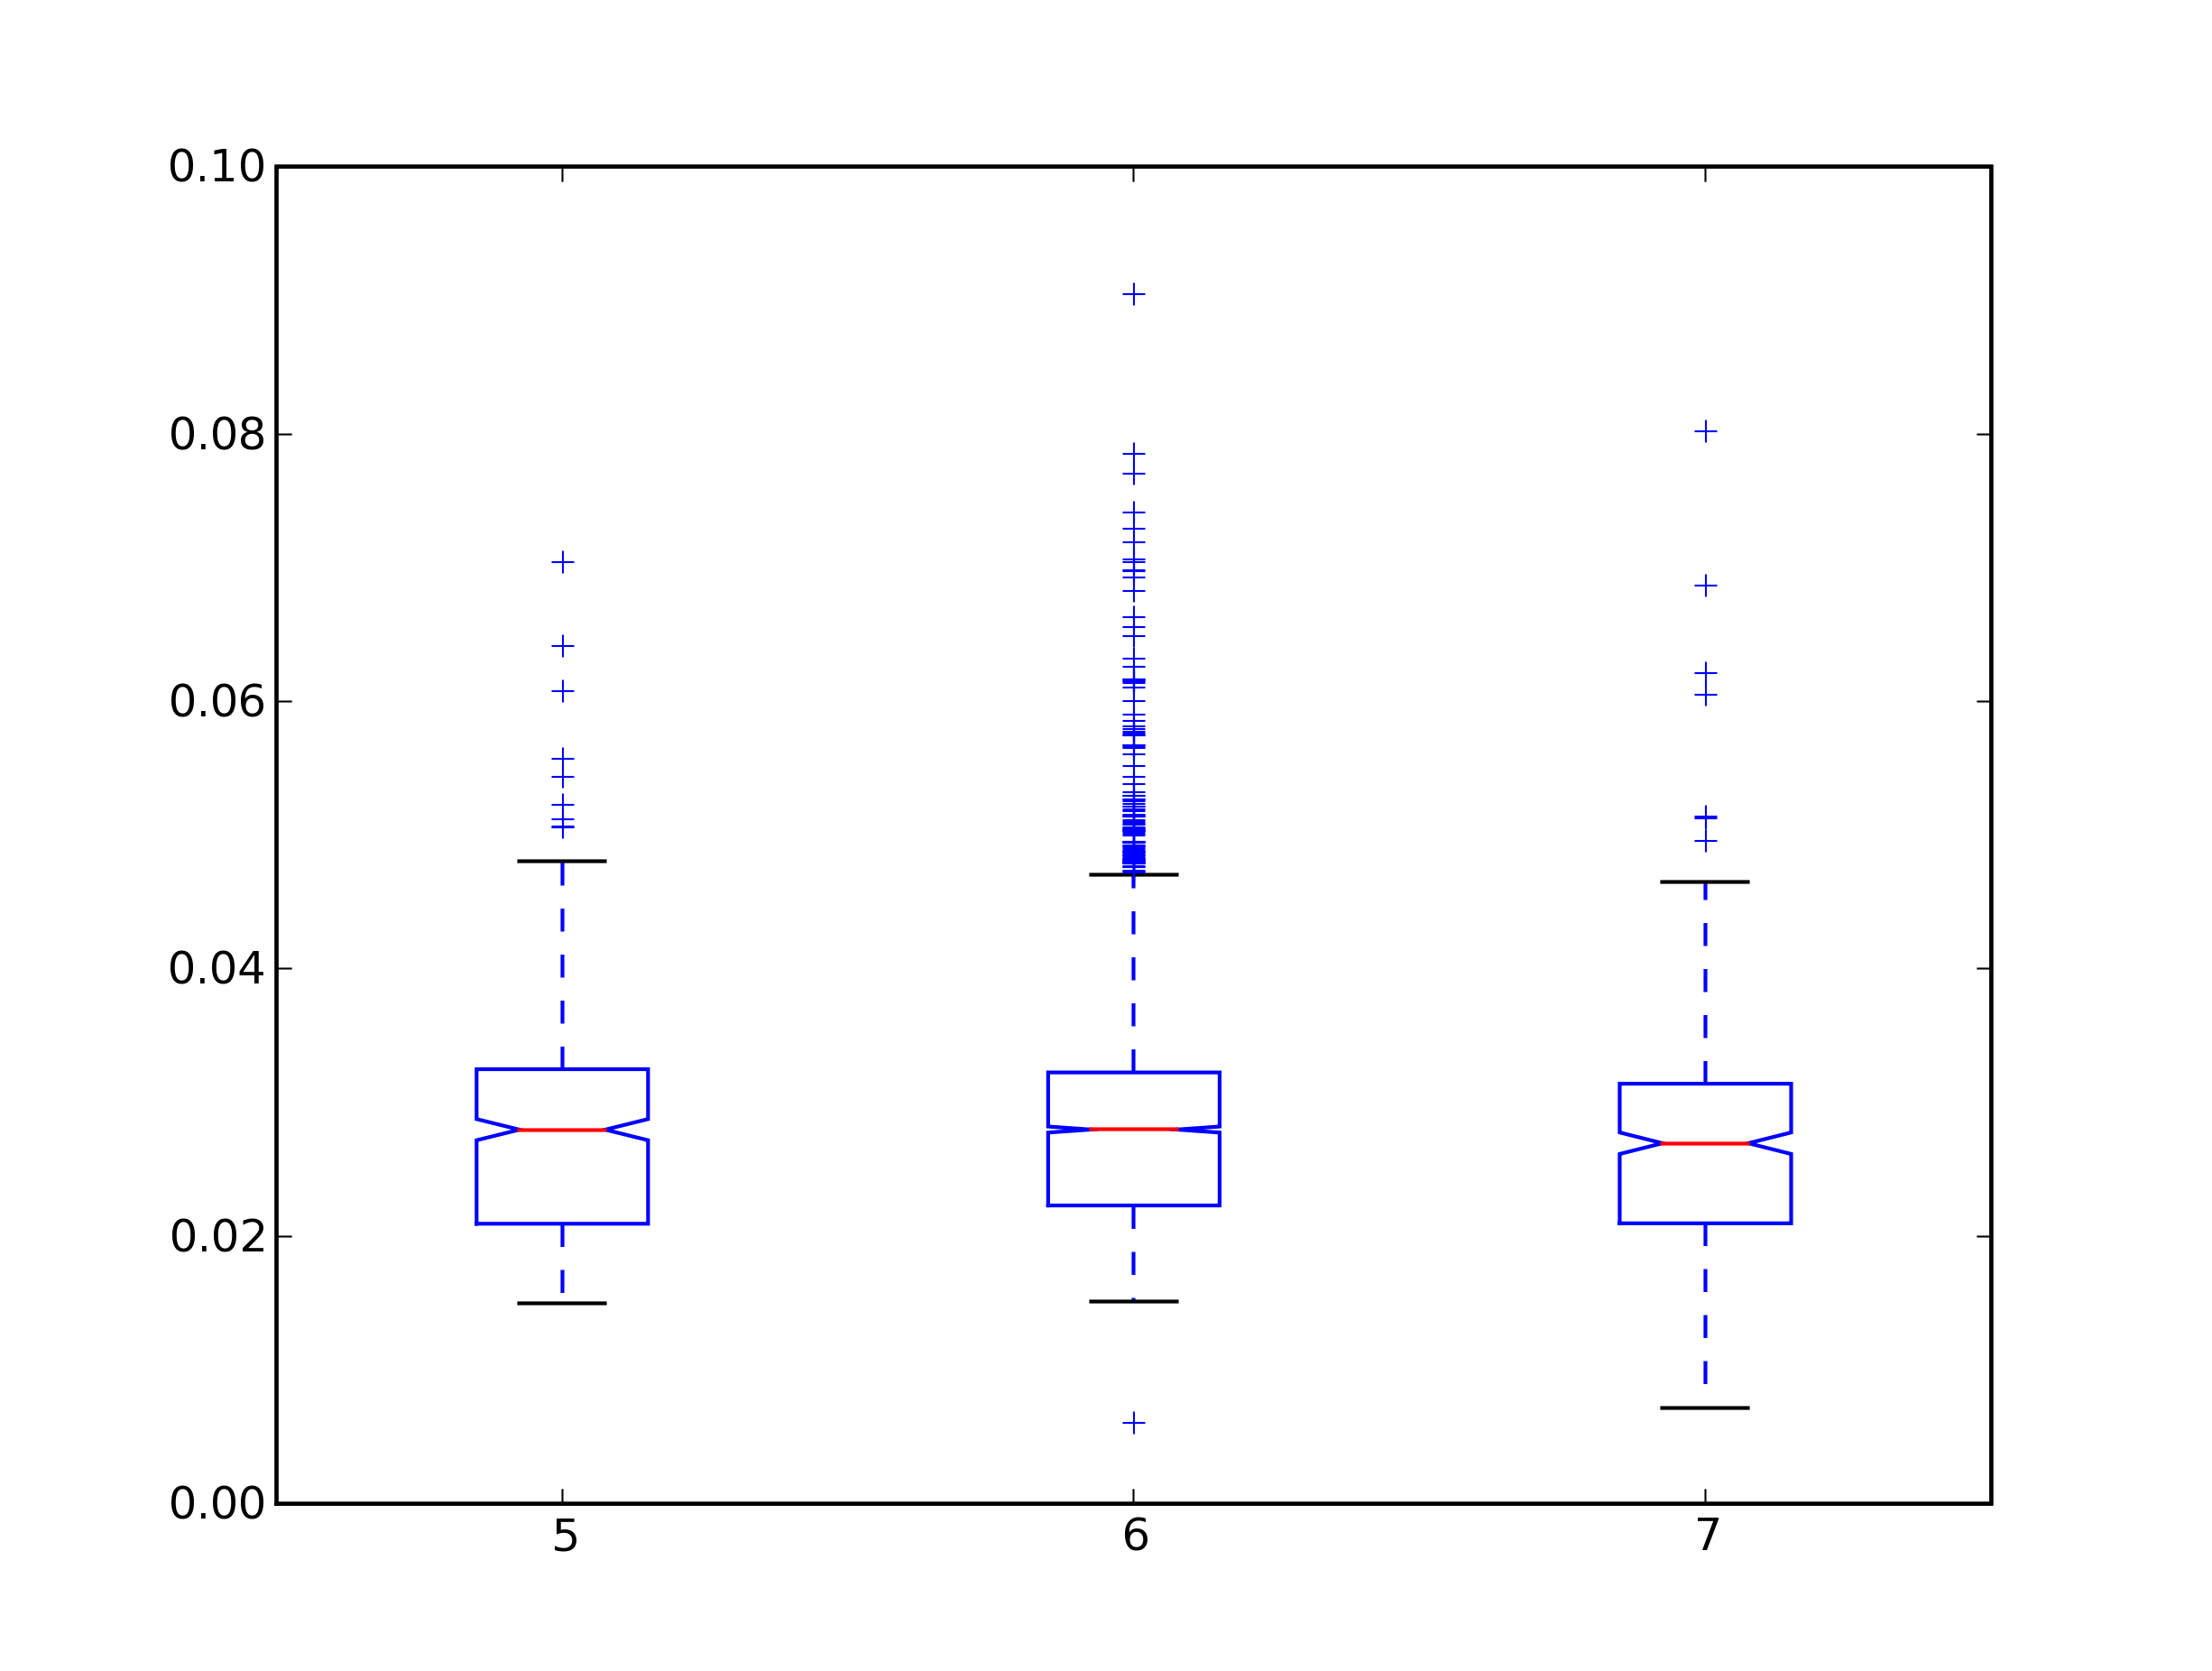
\includegraphics[width=\linewidth]{graph_iv_box.png}
\caption{This shows 4 box plots, each representing one group of neurons in a set
of SOMs trained with the same paremeters.}
\label{fGraphIV}
\end{figure}

\begin{figure}
\centering
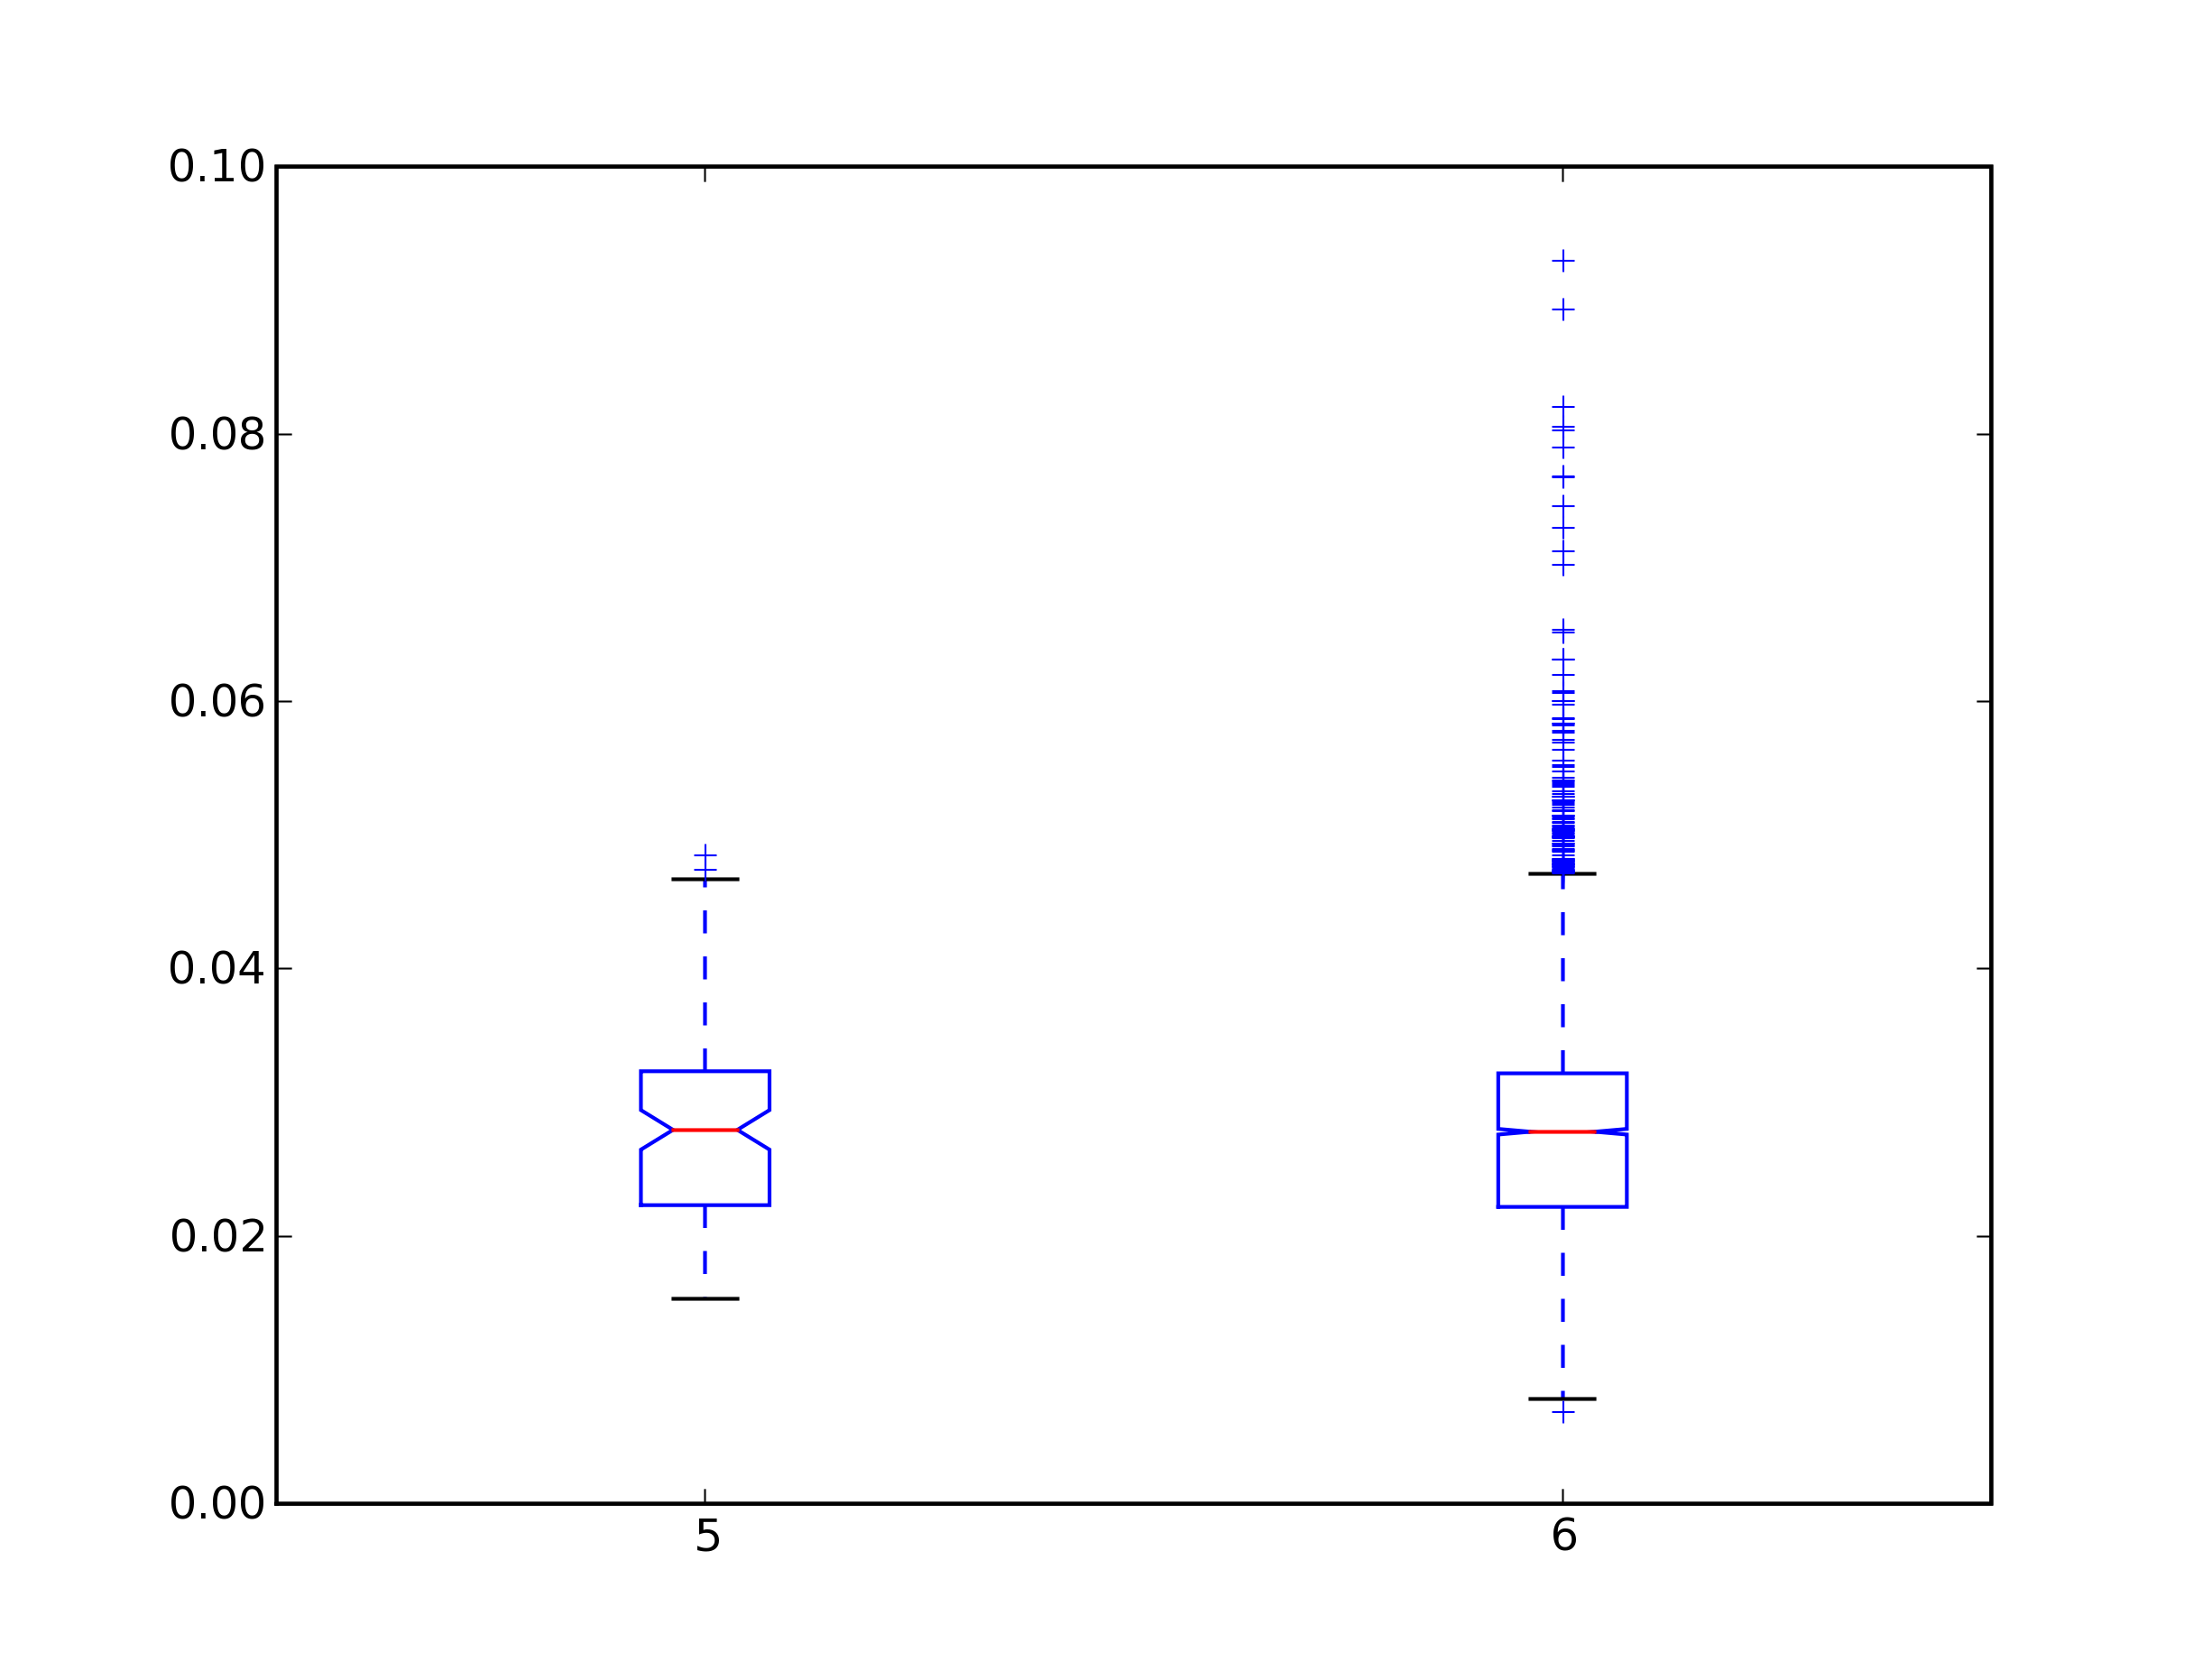
\includegraphics[width=\linewidth]{geodesic_iv_box.png}
\caption{This shows 4 box plots, each representing one group of neurons in a set
of SOMs trained with the same paremeters.}
\label{fGeodesicIV}
\end{figure}




To answer this question we need to setup a distance matrix (the distance of the
means) between each set of groups with in a given topology.  The table should
look like this...... 
\\
  2 3 4\\
2 0 + +\\
3 - 0 +\\
4 - - 0\\
\\
differance of means test\ldots
\ref{randomLabelTableRook}
\ref{randomLabelTableGraph}
\ref{randomLabelTableHex}
\ref{randomLabelTableGeodesic}

\begin{table}
\centering
\caption{Random Labeling Mean Tests for rook case,  delta (p-Value)}
\label{randomLabelTableRook}
\begin{tabular}{|c||c|c|c|}
\hline
&2&3&4\\
\hline
\hline
2& & 0.012681 (0.009000)& 0.024790 (0.001000)\\
\hline
3& 0.012681 (0.011000)& & 0.012109 (0.001000)\\
\hline
4& 0.024790 (0.001000)& 0.012109 (0.001000)& \\
\hline
\end{tabular} \end{table}


\begin{table}
\centering
\caption{Random Labeling Mean Tests for spherical case,  delta (p-Value)}
\label{randomLabelTableGraph}
\begin{tabular}{|c||c|c|c|}
\hline
&5&6&7\\
\hline
\hline
5& & 0.000362 (0.786000)& 0.001358 (0.480000)\\
\hline
6& 0.000362 (0.752000)& & 0.000996 (0.484000)\\
\hline
7& 0.001358 (0.503000)& 0.000996 (0.514000)& \\
\hline
\end{tabular} \end{table}

\begin{table}
\centering
\caption{Random Labeling Mean Tests for Hexgonal Lattice,  delta (p-Value)}
\label{randomLabelTableHex}
\begin{tabular}{|c||c|c|c|c|c|}
\hline
&2&3&4&5&6\\
\hline
\hline
2& & 0.004463 (0.525000)& 0.011735 (0.083000)& 0.017665 (0.011000)& 0.021821
(0.003000)\\
\hline
3& 0.004463 (0.548000)& & 0.007272 (0.006000)& 0.013202 (0.001000)& 0.017357
(0.001000)\\
\hline
4& 0.011735 (0.095000)& 0.007272 (0.002000)& & 0.005930 (0.014000)& 0.010086
(0.001000)\\
\hline
5& 0.017665 (0.012000)& 0.013202 (0.001000)& 0.005930 (0.019000)& & 0.004155
(0.060000)\\
\hline
6& 0.021821 (0.002000)& 0.017357 (0.001000)& 0.010086 (0.001000)& 0.004155
(0.056000)& \\
\hline
\end{tabular} \end{table}

\begin{table}
\caption{Random Labeling Mean Tests for Geodesic Lattice,  delta (p-Value)}
\label{randomLabelTableGeodesic}
\begin{tabular}{|c||c|c|}
\hline
&5&6\\
\hline
\hline
5& & 0.001476 (0.601000)\\
\hline
6& 0.001476 (0.584000)& \\
\hline
\end{tabular} \end{table}






%\chapter{Significance and Limitations}
\chapter{CONCLUSIONS}
The spherical SOM has been widely suggested as a solution to the edge effect
in traditional SOM.  The edge of the traditional SOM is a problem because neurons on
the edge of the topology are less central to the neural network than those in
the center, resulting in differing levels of influence on the
training process.  We extended this problem to spherical SOM by
asserting that irregular spherical topologies will have neurons that are less
central than others.  Existing research in spherical SOM has widely been
focused on minimizing this irregularity and the commonly used tessellated
icosahedron based topology offers the most regular topology. However, the main
disadvantage of this topology type is that it offers very limited control over
network size.  Alternative methods for generating the spherical topology,
which can create a network of any size, have been reviewed or suggested by
\cite{wu2005} and \cite{Nishio:2006fk}.  These alternative methods have been
largely dismissed because they produce network structures that are more irregular.
This research has taken a closer look at the impact that irregularity has on
the training process in an attempt to address the suitability of these less regular
topologies for use in SOM.

The objective of this research was to determine the utility of certain
irregular spherical topologies that offer greater control over
network size.  Toward that end, new diagnostic measures were developed that
allow for SOM comparisons based on topology-induced errors.  The diagnostics
measure the internal heterogeneity of observations captured by a given neuron
relative to that neuron's first-order neighborhood size, as well as relative
to a composite measure of topological regularity.

In this study the new diagnostics were applied to the evaluation of both
traditional and spherical SOMs. Each SOM was trained using the same synthetic
data and training parameters, but utilizing different network topologies.  By
formally testing for difference of means and variance in the results of the
diagnostics, the following conclusions were made: 1) The internal
heterogeneity of a neuron decreases as its first-order neighborhood size
increases, but less so in spherical topologies.  2) The average internal
heterogeneity of a SOM is higher when a more irregular topology is used.  3)
Visualizing internal heterogeneity provides valuable insight into the
underlying training process and how the SOM represents clusters. From these
conclusions, we can make interpretations on the importance of topological
irregularities in SOM.

In comparison to the tradition rectangular and hexagonal topologies, the effects
of irregular topology were minimized in both of the spherical
topologies we tested.  Specifically, we found no significant differences
between the two different spherical topologies we test.  As such, we believe
that the importance of regularity within spherical SOM may be overstated.
Relying only on highly regular spherical topologies may place
unnecessary constraints on the users of spherical SOM.  For example, using less
regular spherical topologies we can overcome the resolution constraint and build
SOMs with any number of neurons.

In pursuit of these findings we built an open source implementation of SOM,
PySOM. This software is capable of training a SOM with an arbitrary
topology.  This allowed us to test the four different topologies presented in
the previous chapters.  Using PySOM, future researchers may train their
SOMs on a variety of different topologies.  We hope that this will enable an
exploratory based approach to help determine the most appropriate topology for
a given research question.


\section{Limitations}
A key limitation of this research is that we only address how topological
regularity effects the SOM.  We do not address how other attributes of the
topology effect the SOM. Specifically, the benefits and/or costs of removing the
edge are unclear.  More research needs to be done in order to determine if spherical SOM
is appropriate for all applications, or under which conditions it becomes
inappropriate.  The edge effect may in fact be useful in identifying outliers.

Our implementation, PySOM, is significantly slower than existing implementations
of the SOM.  As it is currently written it would not be of much use for
extremely large SOMs due to the speed issues.  PySOM currently does not
implement the shortcut winner search described by \cite{Kohonen2000}.  The
shortcut winner search is a method in which an observation only searches the entire
network for its best match once.  On subsequent iterations that particular
observation will only look in the neighborhood of its previous best match. If
the new best match is on the edge of that neighborhood the search radius is
expanded.


\section{Future Directions}
It would be beneficial to expand this research to investigate other aspects of
topology and their effects on the SOM.  The graph structure allows for great
flexibility in testing changes to the topology.  One could construct an
experiment in which individual nodes are removed from the network topology to
determine the impact of an individual neuron.  It could also be beneficial to
test other topologies using the framework laid out by this thesis.

Using spherical SOMs introduces many challenges in terms of visualization,
particularly in projecting spherical SOMs into two-dimensional Euclidean
space.  The random initialization of the SOM results in an arbitrary rotation of
the trained SOM.  It would be helpful when visually comparing two SOMs if they
were both rotated in a consistent fashion. One could accomplish this by identifying
the two most prominent features of the trained SOM and rotating the SOM such
that the most prominent feature is located at $0^\circ$Latitude,
$0^\circ$Longitude and the second most prominent feature is located as far North
as possible. A third feature could be required if the first two are antipodal.
The challenge in this lies in identifying features in the SOM.  A variety of
metrics could be used to rank individual neurons. Alternately, one could cluster
the neurons and use the resulting regions as features.

A number of improvements can be made to PySOM in order to make it of use to
the broader scientific community.  Implementing the shortcut winning search
could dramatically reduce running time.  Python allows for portions of the code
to be written directly in the C programming language.  The highly computational
sections of the code, such as search for the best matching unit, have the
potential to run significantly faster in C.  
The neighborhood search routines can also be optimized. For example, caching the neighborhood around a given neuron
would drastically reduce the number of neighborhood searches but increase the
program's memory requirements.  Perhaps the most useful addition to PySOM would
be a Graphical User Interface (GUI).  A well designed GUI would greatly increase the
accessibility and usability of this code.

Traditionally the geographical sciences have been concerned with identifying and
understanding relationships found in the context of spatial data.  
The existing toolbox for studying these relationships is sizable 
and steadily growing as geographers develop new ways to look at spatial
information.  While the SOM and spherical SOM are a welcome addition to that
toolbox these tools provide much more than a new visualization method or
clustering technique.  Using SOM we can extract spatial representations from
otherwise aspatial data, allowing us to leverage our existing set of
tools on a whole new set of problems.


%\section{Significance}
%The commonly used tessellated icosahedron based topology offers the most regular topology.   However, the main disadvantage of this topology type is that it offers a limited control over network size.  Alternative methods for generating the spherical topology, which can create a network of any size, have been reviewed or suggested by \cite{wu2005} and \cite{Nishio:2006fk}.  These alternative methods produce network structures that are more irregular.  This research will take a closer look at the impact that the irregularity has on the training process in an attempt to address the suitability of these topologies for use in SOM.

%\section{Limitations}
%This research will look at the relationship between regularity in neuron connectedness and the training of a SOM. The relationship between topology and SOM visualization is not addressed. The topology chosen for a SOM has a direct link with how that SOM is visualized.  When representing the topology on the surface of a sphere issues arise with the uniformity in neuron spacing and sizing.  Future work may be needed to address these issues in visualization.


%\subsubsection{Train SOM}

%It is useful to represent our neural lattice as a graph, G.
%We know that any arrangement of neurons onto the surface of a sphere will as such the network can be effectively treated as a graph.  Doing so enables us to use the properties of the graph and the principles of graph theory to help us understand the relationship between neurons during training.

%the variance in neuron spacing should be minimized.    The first condition ensures that each neuron will occupy is only of concern when visualizing the SOM.

%The get at the second condition we must first define the degree of a neuron, deg(n) to be number of its direct neighbors.  Whit that in mind the second condition is that the variance in the degree of the neurons must also be minimized.

%This statement may be somewhat misleading to those investigating alternative 

%For the purpose of SOM visualization it is important for each neuron to receive equal geometrical treatment.

%It is useful to represent the neural network as a graph, G, in order use the...
%In order to examine the irregularities in the neural network it is useful ....

%The basic problem of the ``boundary effect'' is that neurons on the edge have fewer neighbors. Yet there are only five possible arrangements of points on a sphere such that all points have the same number of neighbors.  Any spherical lattice consisting of more then twenty (dodecahedron) neurons will contain topological irregularities.  This is to say that not all neurons will have the same number of neighbors.  The importance of these irregularities and the magnitude of their effects on SOM training is not known.  This goal of this research is to determine whether more flexible network structures may be used in spherical in SOM without introducing significant errors. To accomplish this goal, basic methods in network analysis with be combined with the result from several empirical training runs each utilized different topology.  

%% Note that if you want something in single space you can
% go back and forth between single space and normal space
% by the use of \ssp and \nsp.  If you want doublespacing
% you can use \dsp.  \nsp is normally 1.5 spacing unless you
% use the doublespace option (or savepaper option)

\chapter{INTRODUCTION}
\label{c:intro}

This is the long example thesis produced by the  Department of
Mathematics and Statistics at San Diego State University
as a guide to using the \LaTeX\ template created by the Department.
It complies with the SDSU Thesis Manual produced in 2004
\cite{SDSUthesismanual}. 
The Department has created a \LaTeX\ class file that automatically
handles the formatting requirements of the SDSU Thesis Manual.  The
class file, the source file for this example thesis and for a shorter,
example thesis with more basic information, along with several other
materials are bundled together and available for distribution at
\cite{SDSUMath_thesis}. 

\section{Purpose}
\label{s:purpose}
This document  illustrates some of the more complex typesetting tasks
that are commonly encountered in a thesis containing mathematics.
The student should consult the  short example thesis
accompanying this distribution for information on more basic questions 
concerning the use of \LaTeX. All theses 
must follow the guidelines of the  SDSU Thesis Manual for formating. 
Most formating issues will be automatically handled by the \LaTeX\
class file included with the source file for this document, but there
may be some special circumstances that will require some tinkering
with spacing, pagebreaks, etc.

For a general reference it is recommended that the
student obtain the user's guide and reference manual of Leslie Lamport
\cite{LAM}. Another book that has been recommended is {\em Math into
  \LaTeX\ } \cite{Gra}. 
There are also numerous online resources:  For a general and polished
introduction see \cite{indian_tutorial}; For a focus on mathematics
see \cite{uiuc_tutorial}; For a focus on chemistry and biology see
\cite{microbio_resources}.
 The student should obtain copies of the files used to
generate this document and compare the ASCII source files with 
the \LaTeX\ output.

\section{The long example thesis}
\label{s:long}
The files for this long example
thesis are the following.
\begin{itemize}
\item {\tt sdsu-thesis.cls}: Defines the layout and formatting.
\item {\tt dchem.sty}: A package for doing chemistry.
\item {\tt thesis.tex}: 
\begin{enumerate}
\item  Contains information for the title page, and other
front-matter.
\item Contains a command to include the material from  the files 
{\tt abstract.tex},  {\tt body.tex}, and {\tt append.tex}.
\item Defines the bibliographical style (``plain'' in this example)
  and creates the bibliography using the file {\tt thbib.tex}. 
\end{enumerate}
\item {\tt abstract.tex}: Contains the abstract.
\item {\tt body.tex}: Contains all the text for chapters. 
\item {\tt append.tex}: Contains all the text for appendices.
\item {\tt thbib.bib}:  Contains a bibliographical database.
\item {\tt somb.eps}, {\tt cos.eps}, {\tt plot2.eps}, {\tt
  mol.cloud.ps}:  
Encapsulated postscript files 
that are included by {\tt body.tex}.
\item {\tt Makefile} This can be used on a unix/linux platform to
simplify the processing of \LaTeX/ files.
\end{itemize}

After processing these files the format of the thesis should comply
with the SDSU Thesis Manual.  The numbering of chapters, sections,
theorems, and bibliographical entries and any referencing to these
items should be correct.  Tables and figures are automatically placed
by \LaTeX, subject to certain constraints that you can provide.  
Occasionally, you may find  \LaTeX\ does not break a page or line  you
want it too, or you'd like to add vertical or horizontal space.
The command {\tt $\backslash$hspace\{1in\}} adds horizontal space and
{\tt $\backslash$vspace\{1in\}} adds vertical space.  You may also use
{\tt pt} (points) or {\tt cm} as 
measurements.  The  starred form {\tt $\backslash$hspace*\{12pt\}} of the command
is more persuasive than the unstarred form.  For breaking a line
{\tt $\backslash$newline} or {\tt $\backslash$linebreak} and for
breaking a page {\tt $\backslash$clearpage}, {\tt $\backslash$pagebreak}, {\tt
  $\backslash$newpage} are used, with subtle differences between these
commands (see a good reference). 


\chapter{THE EXCITING WORLD OF EQUATIONS,
THEOREMS, FIGURES AND TABLES}
\label{c:main}
In this chapter we see how equations, theorems,
figures and tables are created, enumerated and referenced.
Each of these items may be given a label
using {\tt $\backslash$label\{<labelname>\}}).
The item can then be referred to by {\tt
$\backslash$ref\{<labelname>\}}).
To see how any one of the examples is created, see the source file {\tt body.tex}.

We also play around with lengths of chapter and section headings.
For example, this chapter begins with a long chapter heading that must conform to the
thesis manual.  Later on there is a very long section heading.  These
examples show how the SDSU thesis class file automatically handles
formating.

We will occasionally refer to the {\it preamble} of the document.
This is set of  lines between the \LaTeX\
commands {\tt $\backslash$documentclass} and {\tt $\backslash$begin\{document\}}.
You may add or alter commands in the preamble to use supplementary
packages.  You can also use commands for a number of other things, as
we describe below.


\section{Equations}
\label{s:equations}
Within a line, mathematics is typeset using two dollar signs, \$, to
enclose the mathematical formula. For example $x_1^2 = x_{i_2}$.
Braces, \{ and \}, are used to help \LaTeX\ parse the input.
For displayed equations you may enclose the material with \verb+\[+
and \verb+\]+.
\[
I^e=\{f\in A\mid
\varphi(f)_i =0\ \forall i \mathrm{\ such\ that\ }
e_i\not=0\}.
\]
You may also use {\tt $\backslash$begin\{equation\}} and  {\tt
  $\backslash$end\{equation\}}. 
Here is a general differential equation,
\begin{equation}
\dot{x} = f(t,x),\qquad x(0)= x_0. \label{de1}
\end{equation}
To see that the numbering is going fine we insert a matrix system as
follows:
\begin{equation}
\dot{y} =
\begin{bmatrix}
a_1 & 0 & \cdots & 0 \\
0 & a_2 & \cdots & 0 \\
\vdots & \vdots & \ddots & \vdots \\
0 & 0 & \cdots & a_n
\end{bmatrix}
y.
\label{de2}
\end{equation}
The numbering is valuable when one wants to refer to the
Equations~(\ref{de1}) and~(\ref{de2}). You may also use abbreviations,
Eqn.~\eqref{de1} and~\eqref{de2}, but you should be consistent
about using one or the other.
Note that when referring to
Eqn.~(\ref{de1}) you must capitalize as we have
and it is best to type 
 a $\tilde{\phantom{x}}$ between the word Eqn., and the reference to avoid
inappropriate division of the label at the end of a line.

Notice that a displayed equation defined using  \verb+\[+ and
\verb+\]+, like the first equation above,  is not numbered. 
One may also  suppress numbering by using the starred form of the
{\tt equation} environment.
{\em e.g.}  {\tt $\backslash$begin\{equation*\}}.
\begin{equation*}
\dot{y} = g(y),
\end{equation*}

There are several other environments for displayed equations (each
having a starred form to suppress numbering). The {\tt align}
environment is useful for multiline equations or formulas.  It  requires an
ampersand in each line and uses it to align the formulas.
Here is the parameterization of the tangent surface to the twisted
cubic curve in 3-space.
\begin{align}
 k[x,y,z] &\longrightarrow k[t,u] \\
x & \longmapsto t + u \notag \\     %notice the placement of \notag
y & \longmapsto t^2 + 2tu \notag \\ %before the \\.
z & \longmapsto t^3 + 3t^2u \notag
\end{align}
Notice that all but the first line have a {\tt $\backslash$notag}
command to suppress numbering. 

There is also an {\tt alignat} environment that allows you to align
more than one equation in a row and add extra space between the equations.
\begin{alignat}{2}
\label{e:rho lam}
\rho(e_i) &= \rho(f_i) & \qquad \lambda(e_i) &= \lambda(f_{i-1}) 
\intertext{I can even add some text between the two rows.}
\rho(e'_i) &= \rho(f'_i) & \qquad \lambda(e'_i) &= \lambda(f'_{i-1}) 
\end{alignat}

Here are a couple of other useful examples
\[
\delta_{ij} = \begin{cases}
1 & \text{if $i=j$} \\
0 & \text{else}
\end{cases}
\]
For $f(x)= \prod_{i=1}^n (x-\alpha_i)$ we have
\[ 
f'(x) = 
\sum_{i=1}^n \prod_{\substack{j=1 \\j \not= i}} ^n (x-\alpha_j)
\]
You might want to label arrows
\[
X \stackrel{f}{\longleftarrow} Y
\]

\section{Theorems, etc.}
\label{s:theorems}
Modern mathematics texts are quite formal about enumerating theorems,
lemmas, definitions etc.  In this 
section we show how to do this with  \LaTeX.

\begin{definition}   
\label{d:stable}
A linear differential equation is asymptotically stable if and only if
all eigenvalues, $\lambda$, of the operator matrix have negative real
part.
\end{definition}
We follow this with a couple of theorems and a corollary.
\begin{theorem}
\label{t:lde}
If the matrix $A$ in the linear differential equation,
\begin{equation}
\dot{y} = Ay, \qquad y(0) = y_0, \label{lde}
\end{equation}
is symmetric, then the solution of {\rm (\ref{lde})} is non-oscillatory.
\end{theorem}
\begin{corollary}
\label{c:symmetric}
If the matrix $A$ in {\rm (\ref{lde})} is symmetric and has negative
eigenvalues, then the solution is non-oscillatory and asymptotically
stable.
\end{corollary}

In order to check how the numbering proceeds we insert here another
theorem.  Notice that Theorem~\ref{t:lde} is the first theorem.
\begin{theorem}
\label{t:antisymmetric}
If the matrix $H$ in the linear differential equation,
\begin{equation}
\dot{y} = Hy, \qquad y(0) = y_0, \label{ldeh}
\end{equation}
is antisymmetric, then the solution of {\rm (\ref{ldeh})} is oscillatory.
\end{theorem}

\begin{proof}
The proof is clear.
\end{proof}

You may choose alternate methods to enumerate theorem-like
environments.  For example, another method would be to use one counter
for all environments.  
In  the preamble at the  beginning of  {\tt thesis.tex} 
you will find the \LaTeX\ code to accomplish this.
You can choose a different method by altering the \LaTeX\ code.
You might also want to add other environments, such as an 
{\em example} environment or an {\em algorithm} environment.
Notice also the {\em proof} environment that nicely places the box at
the end of the proof and introduces the proof with Proof in italic.

\section{Figures or How to Get into Real Trouble if You Take Advantage
of What \LaTeX\ Can Do}
\label{s:figures}

This section shows how to display figures and refer to them in the text.
We will focus here on using \LaTeX\ to insert postscript files using the
{\tt epsfig} package.  Make sure to include
{\tt $\backslash$usepackage\{epsfig\} } in your preamble.

Suppose that we have a postscript file of the  graph of the curve
\begin{equation}
y=\sin(\omega t), \label{gr1}
\end{equation}
where $\omega$ is the circular frequency.
Figure~\ref{fig1} is a graph of Equation~(\ref{gr1}). The interval
of time viewed is $t \in [-5,5]$. The figure reference should be denoted
by either Fig.~\ref{fig1} or by Figure~\ref{fig1}.
\begin{figure}[htb]
\centering
\begin{minipage}{4.5in}
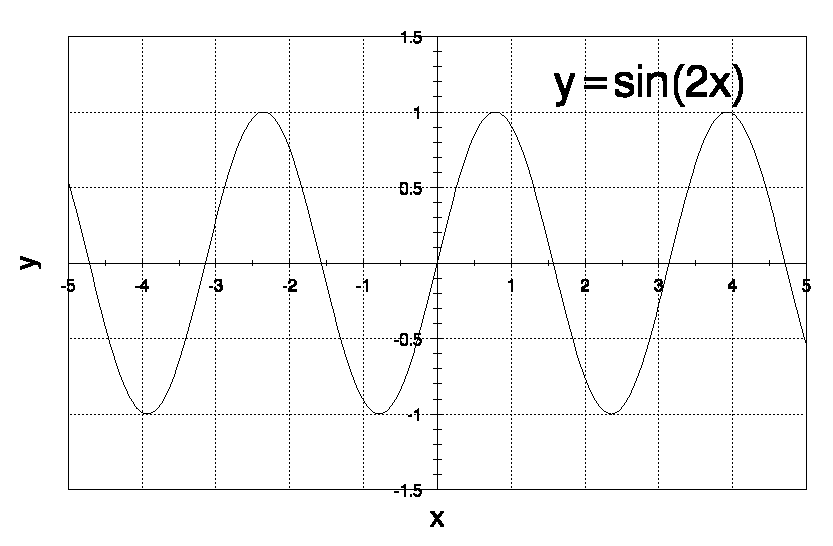
\epsfig{file=plot2.eps,width=4.5in}
\caption{This is a graph of the above equation, where the
circular frequency is taken as $\omega = 2$.\label{fig1}}
\end{minipage}
\end{figure}

This figure was created with a mathematics software package which
produced an encapsulated postscript file.  
In general, to insert  a file named {\tt fname.ps} you
do the following to include it in your thesis:
\\
{ \tt
\hspace*{0.5in} $\backslash$begin\{figure\}[htb]
\\
\hspace*{0.5in} $\backslash$epsfig\{file=fname.ps,height=$x$in\}
\\
\hspace*{0.5in} $\backslash$caption\{Insert a caption here. $\backslash$label\{figlabel\} \}
\\ 
\hspace*{0.5in} $\backslash$end\{figure\}
}
\\
The $x$ above is some number of inches.
This will left justify the figure.  Centering is
a little more complicated and you have to know the width of the figure.
So instead of specifying {\tt height} for the figure we specify
{\tt width}, place everything in a {\tt minipage} environment of that width
and center that.  For example (where $x$ would be some number again):
\\
{ \tt
\hspace*{0.5in} $\backslash$begin\{figure\}[htb]
\\
\hspace*{0.5in} $\backslash$centering
\\
\hspace*{0.5in} $\backslash$begin\{minipage\}\{$x$in\}
\\
\hspace*{0.5in} $\backslash$epsfig\{file=fname.ps,width=$x$in\}
\\
\hspace*{0.5in} $\backslash$caption\{Insert a caption here. $\backslash$label\{figlabel\} \}
\\
\hspace*{0.5in} $\backslash$end\{minipage\}
\\
\hspace*{0.5in} $\backslash$end\{figure\}
}

Fig.~\ref{fullfig} contains two different graphs included in one figure.

Note that if you cannot obtain
postscript figures or are having too much trouble using the technique
described above, then you can use the {\tt $\backslash$vspace}
command to provide an
empty space in the manuscript, then use the old-fashioned technique of
taping in your figure and photocopying it.



%
% If you have oversize full page figures, the following
% might come in handy
%
%\figurecoversheet{\label{figure:oversize} Caption goes here}


%%%%%%%%%%%%%%%%%%%%%%%%%%%%%%%%%%%%%%%%%%%%%%
%%%     The \hspace*{-0.5} moves the figure to the left a bit so that
%%%     it lines up with the caption.
%%%     The \newline seems to be necessary so that the second figure
%%%     lies below the first.
%%%%%%%%%%%%%%%%%%%%%%%%%%%%%%%%%%%%%%%%%%%%%%

\begin{figure}[htb]
\centering
\begin{minipage}{3.5in}
\hspace*{-0.5in}
\epsfig{file=somb.eps,width=3.5in}\newline
\hspace*{-0.5in}
\epsfig{file=cos.eps,width=3.5in}
\caption{The top graph is the function $z = \sin(r)/r$, while
the bottom surface is the function $z = \cos(r)$. \label{fullfig}}
\end{minipage}
\end{figure}

\section{Tables}
\label{s:tables}

The Department of Mathematical Sciences does not have specific
requirements on the exact layout of a table. However, the tables should
be easily readable and properly labeled according to the regulations in
the SDSU Thesis Manual. In this section we want to demonstrate how
\LaTeX\ handles tables. More complicated examples can be found in
Lamport's book \cite{LAM}. We begin with a small table, given by
Table \ref{tab1} which inserts nicely into the text.  Note that the same
centering trick as was employed for figures is done here and we set the
width of the {\tt minipage} environment to 1.9 inches.
%

\begin{table}[hbt]
\centering
\begin{minipage}{1.9in}
 \caption{A Small Table for Listing Some Parameters Used in Some
          Numerical Procedure\label{tab1}}
 \begin{tabular}{|c||c|c|c|c||}    \hline
  Trial &	a  &  b & c & $\omega$ \\ \hline \hline
  1 & 5 & 10  & 15 & $\pi$ \\ \hline
  2 & 10 & 20  & 15 & $2\pi$ \\ \hline
 \end{tabular}
\end{minipage}
\end{table}
%

The manual however allows for the caption to be a little wider if the table
is really small and so we can use a wider {\tt minipage} and then center
the table inside there.  See for example Table \ref{wtab} where we used
width of 3.5 inches.
%
\begin{table}[hbt]
\centering
\begin{minipage}{3.5in}
  \centering
  \caption{Another Small Table for Listing Some Parameters Used in a
           Numerical Procedure\label{wtab}}
   \begin{tabular}{|c||c|c|c|c||}    \hline
    Trial &	a  &  b & c & $\omega$ \\ \hline \hline
    1 & 5 & 10  & 15 & $\pi$ \\ \hline
    2 & 10 & 20  & 15 & $2\pi$ \\ \hline
   \end{tabular}
\end{minipage}
\end{table}

Note that you can use the {\tt center} environment instead of {\tt
$\backslash$centering} but that might add a little bit of unwanted
whitespace.  With {\tt $\backslash$centering} on the other hand, you
might have to put braces around the text you wish to center and
sometimes need to add a {\tt $\backslash$par}.  If you use it inside
a {\tt minipage}, {\tt table} or {\tt figure} environment, you don't have
to really worry about that.  Note however that without the use of
{\tt minipage} you cannot center the caption as it automatically left aligns
itself to conform with the thesis manual.

Tables can also be left aligned see for example Table \ref{ltab}.  Here we
don't use the {\tt minipage} environment, but we must then add linebreaks
so that the table caption does not go wider then the table itself.  We need
to add then two titles, one for the list of tables and one for the caption
here.  The former will not have line breaks and the latter will.
% The first caption (in brackets[]) is used for the list of tables.

\begin{table}[hbt]
 \caption[
   Another such table but left aligned.]{
   Another Such\\Table but Left Aligned\label{ltab}}
 \begin{tabular}{|c||c|c|c|c||}    \hline
  Trial &	a  &  b & c & $\omega$ \\ \hline \hline
  1 & 5 & 10  & 15 & $\pi$ \\ \hline
  2 & 10 & 20  & 15 & $2\pi$ \\ \hline
 \end{tabular}
\end{table}


You might also want to use an entire page for a long table,
This is done by typing the command $\backslash$begin\{table\}[p]. 

Here is an example, included in the minipage environment, to show how 
footnotes\footnote{We also need to see how a regular footnote
appears in the text, so one was inserted here. Multiple lines are easily
handled by \LaTeX.}
can be added to a table.
\begin{table}[bh]
\centering
\begin{minipage}{3.7in}
\caption{Computations for Products of the {\em rrn} Genes at Different
Growth Rates\label{tab2}}
\begin{tabular}{|c||c|c|c|c|c||}	 \hline
 $\tau$(min)  &  100  &	60 & 40 & 30 & 24 \\ \hline \hline
 $C$ period & 67 & 50  & 45 & 43 & 42 \\ \hline
 $D$ period & 30 & 27  & 25 & 24 & 23 \\ \hline
 $V_0$ & 0.437 & 0.577 & 0.815 & 1.15 & 1.63 \\ \hline
 $\bar c$\footnote{$\times 1000\ {\rm ribosomes}/\mu{\rm m}^3$.}
 & 11.1 & 16.8 & 22.1 & 28.1 & 31.4 \\ \hline
$\bar c_{85}$\footnote{$\times 1000\ {\rm ribosomes}/\mu{\rm m}^3$,
representing the average concentration of the product of the {\em rrn} gene
located at $85'$.} & 1.73 & 2.68 & 3.65 & 4.81 & 5.57 \\ \hline
$\bar c_{57}$\footnote{$\times 1000\ {\rm ribosomes}/\mu{\rm m}^3$,
representing the average concentration of the product of the {\em rrn} gene
located at $57'$.} & 1.36 & 1.98 & 2.43 & 2.87 & 2.96 \\ \hline
$\bar c_{85}({\scriptstyle\times 100})/\bar c$\footnote{Percentage of
$\bar c$ produced by the {\em rrn} gene located at $85'$.} & 15.6 & 15.9 &
16.5 & 17.1 & 17.7 \\ \hline
$\bar c_{57}({\scriptstyle\times 100})/\bar c$\footnote{Percentage of
$\bar c$ produced by the {\em rrn} gene located at $57'$.} & 12.3 & 11.8 &
11.0 & 10.2 & 9.44 \\ \hline
$\bar c_{85}/\bar c_{57}$ & 1.27 & 1.35 & 1.50 & 1.68 & 1.88 \\ \hline
 $r$\footnote{Initiations/min/gene.} & 3.75 & 10.27
  & 22.56 & 38.42 & 56.98 \\ \hline
$c_{max}$\footnote{$\times 1000\ {\rm ribosomes}/\mu{\rm m}^3$, representing
the maximum concentration during the cell cycle.} & 11.28 & 17.04
  & 22.33 & 28.36 & 31.77 \\ \hline
$c_{max}/c_{min}$\footnote{Ratio of maximum to minimum concentration
 during the cell cycle.} & 1.041 & 1.036 & 1.027 & 1.024 & 1.026 \\ \hline
\end{tabular}
\end{minipage}
\end{table}

%\clearpage
Sometimes a table might not fit onto a single page, in this case you
must not use the {\tt table} environment, but instead the {\tt longtable}
environment.  Do note that {\tt longtable} automatically centers so you need
not worry about that.  See Table \ref{totallyrandom} for some absolutely
random numbers.  To use the {\tt longtable} environment you must include the
{\tt longtable} package in your preamble.

\begin{longtable}{|l|l|l|}
% You may need to modify the \LTcapwidth if the title wraps too early, or
% if it makes your table too large
%\LTcapwidth=6in
\caption{A Table of Some Totally Random Numbers} \label{totallyrandom} \\

% Here are our column headings
\hline
\multicolumn{1}{|l|}{\textbf{First}} &
\multicolumn{1}{l|}{\textbf{Second}} &
\multicolumn{1}{l|}{\textbf{Third}} \\
\hline \hline
\endfirsthead

% Here is the caption on other pages
\caption*{\tablename\ \thetable{} (continued)} \\
\hline \multicolumn{1}{|l|}{\textbf{First}} &
\multicolumn{1}{l|}{\textbf{Second}} &
\multicolumn{1}{l|}{\textbf{Third}} \\ \hline \hline
\endhead

\multicolumn{3}{r}{\textbf{(table continues)}}
\endfoot

\hline
\endlastfoot

$16883.20050 \times 64.19591$ & $23174^{2905}$ & $(5112,5468,27117)$ \\ \hline
$7216.3398 \times 12239.16770$ & $19961^{9127}$ & $(16136,21997,26051)$ \\ \hline
$15977.29588 \times 5732.19698$ & $14995^{26728}$ & $(28634,14278,17183)$ \\ \hline
$24699.2338 \times 8803.18474$ & $19221^{28853}$ & $(18539,6044,19259)$ \\ \hline
$21444.11156 \times 24727.15793$ & $18372^{28126}$ & $(28032,2375,15319)$ \\ \hline
$4391.18511 \times 4548.30442$ & $1720^{1369}$ & $(3406,21419,16364)$ \\ \hline
$30135.17285 \times 30643.14550$ & $9216^{213}$ & $(23353,27690,19435)$ \\ \hline
$19438.13461 \times 25479.5929$ & $2137^{3868}$ & $(30657,17930,22240)$ \\ \hline
$26015.13194 \times 24615.8566$ & $17585^{10358}$ & $(13114,15259,12079)$ \\ \hline
$14483.18666 \times 730.30848$ & $16033^{18015}$ & $(28723,30583,27231)$ \\ \hline
$28936.21168 \times 22153.15603$ & $7838^{2847}$ & $(8315,13767,4984)$ \\ \hline$12183.11656 \times 22915.1655$ & $4903^{3341}$ & $(26271,13469,20927)$ \\ \hline
$3861.26584 \times 3418.15940$ & $8299^{22084}$ & $(16670,6379,5349)$ \\ \hline
$1917.2334 \times 3164.29148$ & $31271^{24332}$ & $(18534,14106,32170)$ \\ \hline
$21381.22421 \times 13170.26365$ & $1836^{24826}$ & $(16512,3492,29730)$ \\ \hline
$19854.29763 \times 10431.8013$ & $856^{4247}$ & $(11431,16797,12547)$ \\ \hline$748.699 \times 18926.6097$ & $2617^{21261}$ & $(9262,31765,19764)$ \\ \hline
$826.17531 \times 1102.229$ & $6144^{23524}$ & $(13399,32510,25360)$ \\ \hline
$5457.16254 \times 28852.2419$ & $3340^{25847}$ & $(12851,11353,26704)$ \\ \hline
$17098.22785 \times 10733.29645$ & $23533^{11432}$ & $(15804,29630,14049)$ \\ \hline
$4297.6124 \times 13047.24061$ & $6951^{30578}$ & $(25163,7180,3955)$ \\ \hline
$15919.20579 \times 3697.8512$ & $26036^{19951}$ & $(4596,28456,23292)$ \\ \hline
$30444.8539 \times 1877.24380$ & $25637^{24662}$ & $(2345,22515,15427)$ \\ \hline
$13777.5551 \times 12290.27827$ & $9848^{18414}$ & $(8106,1141,25365)$ \\ \hline$5916.26304 \times 32545.9871$ & $9456^{20356}$ & $(13568,17968,13625)$ \\ \hline
$752.22564 \times 9313.24044$ & $20240^{17852}$ & $(25921,11852,10721)$ \\ \hline
$17816.14197 \times 468.475$ & $27975^{6019}$ & $(12765,23034,15867)$ \\ \hline
$31180.31140 \times 17008.23777$ & $4288^{10545}$ & $(23555,14160,20001)$ \\ \hline
$11143.27728 \times 5201.24768$ & $28480^{27765}$ & $(1313,19756,15238)$ \\ \hline
$19165.12910 \times 27090.29887$ & $30726^{8520}$ & $(30355,31201,3727)$ \\ \hline
$3607.11199 \times 26761.19474$ & $9611^{25133}$ & $(3715,620,29421)$ \\ \hline
$14260.24175 \times 10813.1493$ & $2551^{5774}$ & $(6694,27319,1486)$ \\ \hline
$1691.28633 \times 21243.16929$ & $15030^{1385}$ & $(11252,12149,32111)$ \\ \hline
$19772.9737 \times 30544.23499$ & $13344^{8975}$ & $(17492,50,18586)$ \\ \hline
$9857.3765 \times 19207.6510$ & $18025^{10614}$ & $(17324,19518,13165)$

\end{longtable}


\chapter{CREATING A BIBLIOGRAPHY USING {\sc Bib}{\TeX} }
\label{c:biblio}
There are two ways to create a bibliography.  In the short example
thesis you enter the bibliographic items as they are supposed to
appear.  In this example thesis we show how to use {\sc Bib}\TeX.
With {\sc Bib}\TeX\ you create a separate file, {\tt thbib.bib} in our
example, containing data about each bibliographical item.
Here is an example,
\begin{verbatim}
@article{ART,
  author="Abraham, T.",
  title="Mathematical study of $\gamma$-rings in a {H}ilbert space",
  journal="J. Math. Anal. Appl.",
  volume="19",
  pages="125-128",
  year="1984"
}
\end{verbatim}
Here {\tt @article} describes the type of entry and {\tt ART} is the
tag that you use to cite the entry.
Running {\sc Bib}\TeX creates a file containing your bibliography in
\LaTeX\ format, {\tt thesis.bbl} in this example.  
You don't have to worry about alphabetizing,
enumerating, or  formatting. {\sc Bib}\TeX\ does all of that
automatically.  Furthermore, {\sc Bib}\TeX\ only includes items that
you have referenced in the thesis, so your database can include
extraneous entries.  {\sc Bib}\TeX\ also allows you to choose the 
bibliographical style  with one command, for example
{\tt \verb+\bibliographystyle{plain}+}, so it is easy to change from
one style to another.

MathSciNet has a nice feature that frees you from actually entering
the data. 
If you do a search for the item on MathSciNet, you will see a button
that says ``select alternative format.''  Choose {\sc Bib}\TeX\ and
you will get the bibliographical data.
There is also a clipboard on the  search page on which you can
store  data for several items.  Click ``Add citation to
clipboard'', below each item that you want.
You can see the items you've selected by clicking  on the link "View
clipboard" at the top left of  the page.
Select ``Bibtex'' as format, hit the ``Text'' button and you have the
data.  You will probably want to change the tags to something easy for
you to remember.

In the bibliographic database we have included  references for journal articles
\cite{ART}, books and booklets \cite{AM,BKL}, chapters or articles in
books, collections, and proceedings \cite{INB,INC,INP}. 
Other sources may be proceedings \cite{PRO},
technical reports \cite{TEC}, theses \cite{MTH}, or unpublished material
\cite{UNP}.  A number of online references are also given
\cite{uiuc_tutorial,indian_tutorial}.
This should provide a fairly comprehensive list for any
material that the student may encounter.  For additional assistance, see
the graduate adviser in your area of concentration.  

When you want to include a reference to a particular page, theorem
chapter or whatever, you can use an optional argument to the cite
command.  For example, \cite[Thm.~1.1]{AM}


\chapter{CHEMISTRY}
\label{c:chem}

For chemistry theses with many mathematical formulas, the 
{\tt   amsmath} package is  recommended. Simply use the line
{\tt $\backslash$usepackage\{amsmath\}} in the preamble.

To obtain the {\sc Bib}\TeX\ style file for formatting references in ACS style,
install the  following package.
\begin{description}
\item \verb+http://www.ctan.org/tex-archive/macros/latex/contrib/achemso+
\end{description}
Although providing limited support for ACS manuscript submissions,
it does not include any tools for writing chemical reactions, much less
chemical structures.

There are additional chemistry style files available on CTAN to assist
in drawing structures and writing formulas, but it is not clear to what
extent there is continuing support for these.  See, for example,
\begin{itemize}
\item Chemical formulas with \LaTeX:\\
\verb+www.ctan.org/info?id=ochem+
\item Chemical formulas and equations:\\
\verb+http://www.ctan.org/info?id=mhchem"mhchem+
\item Structural organic chemistry:\\
\verb+www.ctan.org/info?id=streetex+
\item Chemical structures:\\
\verb+www.ctan.org/info?id=xymtex+
\end{itemize}

There is also a program for  writing chemical equations and getting
chem-specific symbols,  by Donald Arsenau.  
Arsenau allows this to be freely distributed (providing it is not altered), 
but has not yet posted it to CTAN.  
We have included it in  this distribution. 

Given the graphical demands of typical publications in synthetic chemistry,
it is probably wiser to rely on a more powerful graphics program like 
ChemDraw to prepare the graphic, and then import that into the
LaTeX document with psfig (for postscript figures) or similar graphics 
package.
  
In the next section  we give some examples that show how to use the
{\tt  rxnarray } 
environment, standard state symbols, and subscript and superscript placement 
with {\tt dchem.sty}.  It also shows how to  import a postscript
figure using psfig and the align environment from the amsmath package.  

\section{An example}
\label{s:chem}
Hydrogen molecules on the fringe of a molecular cloud occasionally
collide with atoms from the neighboring warm regions.  Those molecules in
turn collide with other molecules, and heat up the molecular cloud.
However, when one of the fast-moving $\ch H_2$ molecules collides with
CO or HCN, these will often be left in excited rotational states.
Unlike $\ch H_2$, which has no permanent dipole moment, CO and HCN have
allowed rotational transitions.  The $N = 1\rightarrow 0$ transition
of CO, for example, is at 3.3 cm$^{-1}$.  What this implies is that
emission lines are available for the molecular clouds even at
energies corresponding to only a few K in temperature.  Consequently,
the molecular clouds can get much colder than the atomic gas
(Fig. \ref{fig-mol.cloud})\footnote{Notice that this is a small figure
  with a very  long caption.  The thesis manual allows for the caption to be
 wider than a figure which is very small.  It also
 allows for a very long  caption to run the width of the page.}
.

 \begin{figure}[t,b,h,p] 
  \par\hbox
  {
   \hspace{2in}
   \vbox
   {
    \vspace{0.1in} \psfig{figure=mol.cloud.ps,height=1.5in}
   }
  } 
  \caption{\
Molecular clouds are cooler
 than the surrounding atomic gas, as low as 5 K, because
 they constantly emit radiation from rotational transitions
 of polar molecules into the optically thin surroundings.
 No significant cooling transitions are available
 for the atomic gas until its temperature exceeds about 100 K.
{\label{fig-mol.cloud}}} 
 \end{figure}

Consider the following proposed mechanism for the synthesis of
interstellar $\ch c-C_3H_2$ (cyclopropadiene):
\begin{rxnarray}
\label{C2H2+C+}
C^+ ~+~ C_2H_2 & ~\yields~ & \mbox{c-}C_3H^+ ~+~ H \\
\mbox{c-}C_3H^+ ~+~ H_2 & ~\yields~ &  \mbox{c-}C_3H_3^+ ~+~ {\ma h\nu} \\
\mbox{c-}C_3H_3^+ ~+~ e^- & ~\yields~ & \mbox{c-}C_3H_2 ~+~ H
\end{rxnarray}
 The chain of events is spurred by the entrance of a carbon atomic
 ion into a region of stable molecules such as $\ch C_2H_2$ and $\ch H_2$.
 The first step, formation of the cyclic $\ch C_3H^{+}$ ion, has
 an advantage over reactions between neutral molecules:
 the monopole-induced dipole interaction is powerful enough
 at these low temperatures to increase the collision frequency
 of ions and neutrals.   Furthermore, the reaction probability is
 increased over those of typical stable reactants by the very low
 $\Delta H\ts$ associated with free radical reactants such as the 
 open-shell $\ch C^+$ ion.  
The free energy change $\Delta G\stst$ is
 large and negative.

Estimate the rates of formation of HCl$^+$ and HCl at 80 K
in the Orion Molecular Cloud from the reactions given on the preceding page.

\begin{rxnarray*}
Cl^+ ~+~ H_2 &~\eqbm^{\ma k_1}_{\ma k_{-1}}~ HCl^+ ~+~ H \\
Cl   ~+~ H_2 &~\yields^{\ma k_2}~ HCl   ~+~ H
\end{rxnarray*}

\begin{align}
k_1 &= A_1 e^{-E_{a1}/RT} = 1\cdot 10^{-9} ~\mbox{cm$^3$ s$^{-1}$} \\
k_2 &= A_2 e^{-E_{a2}/RT} = 1.3\cdot 10^{-25} ~\mbox{cm$^3$ s$^{-1}$}
\end{align}


%
% The bibliography page, must be between main body and appendices
%
% You must have thbib.bib file in the current directory 
%
%\bibliographystyle{plain}
\bibliographystyle{apalike}
\bibliography{../bib/som}

% This includes append.tex
%\appendices
%
% If you only have one appendix, you should change the above to:
%\appendix
%

\chapter{MORE INFORMATION ON EQUATIONS}

To demonstrate how an appendix should be inserted into the thesis
we have provided two appendices. This first appendix illustrates some
more advanced techniques to improve the appearance of your equations.
Below is a system of partial differential equations from a model for
cellular control by an external nutrient. The equations are complicated
and \LaTeX\ tends to allow them to run into each other. To prevent this
additional spacing between lines is achieved by using 
{\tt $\backslash\backslash$[3pt]} at the end of a line.  
Not also the use of the {\tt $\backslash$dfrac} command for fractions
in displayed equations.
The system is numbered only once by (\ref{sys2}), and
this is centered as best we can on one line.  The other lines have a
{\tt $\backslash$notag} command to suppress numbering.
\begin{align}
  \dot{U}_1(t) & = \tilde f(W_1(t-T)) - U_1(t) + \gamma_1U_2(R\sigma,
   t),	\notag \\[3pt]
  \dot{W}_1(t) & =  -\hat b_3W_1(t) + \gamma_3W_2(R\sigma,
   t),\notag \\[3pt]
  \frac{\partial U_2}{\partial t} & =  D_1\nabla^2U_2 - U_2 - \tilde f(W_1
    (t-T)) - \gamma_1U_2(R\sigma,t){\vrule width 0in depth .1in},
	\label{sys2} \\[3pt]
  \frac{\partial V_2}{\partial t} & =  D_2\nabla^2V_2 - b_2V_2 + c_0
    \bigl(U_2 + U_1(t)\bigr), \\[3pt]
  \frac{\partial W_2}{\partial t} & =  D_3\nabla^2W_2 - b_3W_2 + (\hat b_3
    -b_3)W_1 - \gamma_3W_2(R\sigma,t) \\
    &  \quad + k\left[\left[{\left(\frac{D_3}{r^2}\right)}\frac{d}{dr}\left(r^2
	   \frac{dh}{dr}\right) - b_3h\right]V_2(R,t) - h\dot V_2(R,t)
	   \right], 
\end{align}
For $t > 0$ and $R\sigma < r < R$ and with the boundary conditions:
\begin{align*}
 \dfrac{\partial U_2(R\sigma,t)}{\partial r} & = 
 \beta_1U_2(R\sigma,t), & 
 \dfrac{\partial U_2(R,t)}{\partial r} & =  0, \\
 \dfrac{\partial V_2(R\sigma,t)}{\partial r} & =  0, &
 \dfrac{\partial V_2(R,t)}{\partial r} & =  0,  \\
 \dfrac{\partial W_2(R\sigma,t)}{\partial r} & = 
   \beta_3W_2(R\sigma,t), & 
 \dfrac{\partial W_2(R,t)}{\partial r} & =    0.
\end{align*}

In algebra, one often uses commutative diagrams.  The packages
{\tt amscd}, {\tt diagram} and {\tt xypic} allow you to create
something like the following diagram below.
The {\tt xypic} package is by far the most powerful.
\begin{equation}
\xymatrix{
 X \times_Z Y \ar[d]^q \ar[r]_p & X \ar[d]_f       \\ 
 Y \ar[r]^g   & Z  
}
\end{equation}


The appendix can also include technical theorems and lemmas which are
call in the same manner as before. For example,
\begin{theorem}
The system of equations {\rm (\ref{sys2})} can exhibit periodic
solutions for certain parameter values.
\end{theorem}

\begin{proof}
The argument uses Hopf bifurcation techniques and is very
complicated. See Mahaffy {\it et al} \cite{MJV}.
\end{proof}

\chapter{LISTS AND QUOTATIONS}

To create a list you will want to use one of {\it itemize, enumerate, or
description}. For example:
\begin{description}
\item[continuous] A function $f$ is {\bf continuous} at $x$ if and only
if for every $\varepsilon >0$ there exists a $\delta(x) >0$ such that
whenever $|y-x|<\delta$, $|f(y)-f(x)| < \varepsilon$.
\item[uniformly continuous] A function $f$ is {\bf uniformly
continuous} if and only if for every $\varepsilon >0$ there exists a
$\delta >0$ such that whenever $|y-x|<\delta$, $|f(y)-f(x)| <
\varepsilon$ independent of $x$ and $y$.
\item[equicontinuous] A family of functions $f_n$ is {\bf
equicontinuous} at a point $x$ if and only if for every $\varepsilon >0$
there exists a $\delta >0$ such that whenever $|y-x|<\delta$,
$|f_n(y)-f_n(x)| < \varepsilon$ for all functions $f_n$.
\end{description}

\LaTeX\ provides an environment for block quotations. To agree with the
thesis manual follow the format below for a quotation exceeding four
lines. From Lewis Carrol's {\it Hunting of the Snark} we hear the
Bellman tell his crew:
 \vspace{.12pt}

{
\ssp
\begin{verse}
The Bellman himself they all praised to the skies--\\
Such a carriage, such ease and such grace!\\
Such solemnity, too! One could see he was wise,\\
The moment one looked in his face!\\
 \vspace{.15in}
He had bought a large map representing the sea,\\
Without the least vestige of land:\\
And the crew were much pleased when they found it to be\\
A map they could all understand.\\
 \vspace{.15in}
``What's the good of Mercator's, North Poles and Equators,\\
Tropics, Zones, and Meridian Lines?''\\
So the Bellman would cry: and the crew would reply,\\
``They are merely conventional signs!''\\
 \vspace{.15in}
``Other maps are such shapes, with their islands and capes!\\
But we've got our brave Captain to thank''\\
(So the crew would protest) ``that he's bought us the best--\\
A perfect and absolute blank!''\\
\end{verse}
}



%
% Make the library abstract page
%
%\begin{libraryabstract}
% This just inserts the the abstract.tex file
%% You insert your abstract in the space below.


This document is intended to help students at San Diego State
University to use  \LaTeX\ to produce a Master's Thesis with
high-quality typesetting. Instructions are given for typesetting
complex mathematics and chemical formulas, formatting theorems, using a
variety of table formats, handling figures, and using {\sc Bib}\TeX.  




%\end{libraryabstract}

\end{document}
